\documentclass[11pt,a4paper]{article}
\usepackage[utf8]{vietnam}
\usepackage[left=3.5 cm,right=2 cm,top=3.5 cm,bottom=3 cm]{geometry}
\usepackage{amsmath}
\usepackage{amsfonts}
\usepackage{amssymb}
\usepackage{enumerate}
\usepackage{indentfirst}
\usepackage{rotating}
\usepackage{graphicx}
\usepackage{amsbsy}
\usepackage{epsfig}
\usepackage{listings}
\usepackage{pdfpages}
\usepackage{multicol}
\usepackage[pdftex, % Sử dụng PDF TeX
bookmarks=true, % Tạo bookmarks trong tập tin PDF
pdfencoding=auto, % Tự động điều chỉnh encoding của PDF
unicode=true, % Sử dụng Unicode
pdffitwindow=true, % Fit cho vừa cửa sổ
pdfstartview={FitH}, % Zoom file PDF cho vừa khít với nội dung
]{hyperref}
%\usepackage{subfigure} %không sử dụng cùng subcaption
\usepackage{subcaption}
\usepackage{multimedia}
\usepackage{boxedminipage}
\usepackage{tikz}
\usepackage{nicefrac}
\usepackage{xcolor}
\usepackage{url}
\usepackage{lipsum} %just for the example
\usepackage{fancyhdr}
\usepackage{multirow}
\usepackage{tikz}
\usepackage{scrextend}
\usepackage{titlesec}
\usepackage{mdframed}
%\usepackage{natbib}
\graphicspath{ {figures/} }
\usepackage{array}
\usepackage{biblatex}
\newtheorem{proposition}{Mệnh đề}[section]
\newtheorem{theorem}{Định lý}[section]
\newtheorem{lemma}{Bổ đề}[section]
\newtheorem{corollary}{Hệ quả}[section]
\newtheorem{conjecture}{Dự đoán}[section]
\newtheorem{remark}{Chú ý}[section]
\newtheorem{example}{Ví dụ}
\newtheorem{problem}{Bài toán}[section]
\newtheorem{exercise}{Bài tập}
\newtheorem{define}{Định nghĩa}[section]
\makeatletter
%\usepackage{utopia}
\pagestyle{fancy}
\lhead{\textbf{TIỂU LUẬN}}
\chead{}
\rhead{\textit{\textit{GVHD: TS. Đoàn Duy Trung}}}
\lfoot{\textit{SV. Nguyễn Hữu Thuật}}
\cfoot{}
\rfoot{\thepage}
\renewcommand{\headrulewidth}{0.4pt}
\renewcommand{\footrulewidth}{0.4pt}
\usetikzlibrary{calc}

%% Độ thụt
%%% Của các dòng
\setlength{\parindent}{0pt}

%% Đóng khung văn bản
\newmdenv[linecolor=black,skipabove=\topsep,skipbelow=\topsep,
leftmargin=-5pt,rightmargin=-5pt,
innerleftmargin=5pt,innerrightmargin=5pt]{mybox}
%%===============



\numberwithin{equation}{subsection}
\numberwithin{figure}{subsection}
\numberwithin{table}{subsection}

\begin{document}
\begin{titlepage}
\begin{tikzpicture}[remember picture,overlay,inner sep=0,outer sep=0]
     \draw[blue!70!black,line width=4pt] ([xshift=-1.5cm,yshift=-2cm]current page.north east) coordinate (A)--([xshift=1.5cm,yshift=-2cm]current page.north west) coordinate(B)--([xshift=1.5cm,yshift=2cm]current page.south west) coordinate (C)--([xshift=-1.5cm,yshift=2cm]current page.south east) coordinate(D)--cycle;

     \draw ([yshift=0.5cm,xshift=-0.5cm]A)-- ([yshift=0.5cm,xshift=0.5cm]B)--
     ([yshift=-0.5cm,xshift=0.5cm]B) --([yshift=-0.5cm,xshift=-0.5cm]B)--([yshift=0.5cm,xshift=-0.5cm]C)--([yshift=0.5cm,xshift=0.5cm]C)--([yshift=-0.5cm,xshift=0.5cm]C)-- ([yshift=-0.5cm,xshift=-0.5cm]D)--([yshift=0.5cm,xshift=-0.5cm]D)--([yshift=0.5cm,xshift=0.5cm]D)--([yshift=-0.5cm,xshift=0.5cm]A)--([yshift=-0.5cm,xshift=-0.5cm]A)--([yshift=0.5cm,xshift=-0.5cm]A);


     \draw ([yshift=-0.3cm,xshift=0.3cm]A)-- ([yshift=-0.3cm,xshift=-0.3cm]B)--
     ([yshift=0.3cm,xshift=-0.3cm]B) --([yshift=0.3cm,xshift=0.3cm]B)--([yshift=-0.3cm,xshift=0.3cm]C)--([yshift=-0.3cm,xshift=-0.3cm]C)--([yshift=0.3cm,xshift=-0.3cm]C)-- ([yshift=0.3cm,xshift=0.3cm]D)--([yshift=-0.3cm,xshift=0.3cm]D)--([yshift=-0.3cm,xshift=-0.3cm]D)--([yshift=0.3cm,xshift=-0.3cm]A)--([yshift=0.3cm,xshift=0.3cm]A)--([yshift=-0.3cm,xshift=0.3cm]A);
\end{tikzpicture}
\thispagestyle{empty}
\begin{center}
	\Large
	\textbf{TRƯỜNG ĐẠI HỌC BÁCH KHOA HÀ NỘI}
	
	\vspace{0.1cm}
	\Large
	\textbf{VIỆN TOÁN ỨNG DỤNG VÀ TIN HỌC}
	
	\vspace{1.2 cm}
	\begin{center}
	
\includegraphics[width=2.5 cm]{logo_Hust.png}
	\end{center}	
	
	\vspace{1cm}	
	\Large
	\textbf{HỆ THỐNG HỌC SÂU PHÂN TÁN}
	
	\vspace{1cm}	
	\LARGE
	\textbf{TIỂU LUẬN}\\
	
	\vspace{1 cm}
\Large	\textbf{Môn học: TÍNH TOÁN SONG SONG}
	
	\vspace{0.5 cm}
	\Large \textbf{Chuyên ngành: TOÁN TIN}
	
	\end{center}
	\vspace{1.4cm}	
\begin{center}
\begin{tabular}{ll}
\Large \textbf{Giảng viên hướng dẫn:}  &  \Large \textbf{TS. ĐOÀN DUY TRUNG}\\[0.5 cm]
\Large \textbf{Sinh viên thực hiện:} & \Large \textbf{NGUYỄN HỮU THUẬT}\\[0.5 cm]
\Large \textbf{Lớp:} & \Large \textbf{Toán Tin 01 - K63}
\end{tabular}
\end{center}

	\begin{center}
	\vspace{2cm}
	\Large  \textbf{HÀ NỘI - 2021}
	\end{center}
\end{titlepage}	
	\newpage
%%======================================

\begin{center}
\LARGE \textbf{Lời cảm ơn} \\[0.5 cm]
\end{center}

 Em xin được gửi lời cảm ơn chân thành tới  \textbf{TS. Đoàn Duy Trung} đã tận tình hướng dẫn em trong quá trình học tập và nghiên cứu tại học phần Tính toán song song cũng như trong suốt quá trình học tập tại Viện Toán ứng dụng và Tin học. \\

Em trân trọng gửi lời cảm ơn đến Ban Lãnh đạo trường Đại học Bách khoa Hà Nội, Viện Toán ứng dụng và Tin học đã tạo mọi điều kiện thuận lợi nhất để chúng em có điều kiện hoàn thành học phần một cách an toàn và hiệu quả trong điều kiện tình hình dịch bệnh Covid đang diễn biến hết sức phức tập (tháng 07 năm 2021)..\\

Mặc dù đã rất cố gắng, nhưng vì điều kiện thời gian cũng như kiến thức của bản thân còn hạn chế nên bài tiểu luận không tránh khỏi những sai sót. Em rất mong muốn nhận được sự đóng góp của thầy để em được bổ sung kiến thức và rút kinh nghiệm ở các bài báo cáo sau.\\
%%=============
\begin{center}
\LARGE \textbf{Tóm tắt nội dung tiểu luận}\\[0.5 cm]
\end{center}

Nội dung của tiểu luận được tìm hiểu từ một số bài báo nổi tiếng về đào tạo mô hình học sâu phân phối. Ngoài ra, không thể thiếu là nguồn Internet với những thông tin được cập nhật thường xuyên hơn. Ngoài ra, do hạn chế về điều kiện phần cứng nên chương trình trong bài tiểu luận chỉ mang tính demo và chưa thể hiện được sự hiệu quả của phương pháp này. Tuy nhiên, để khắc phục điều đó, em đã trích dẫn một số kết quả từ các bài báo nhằm nêu bật được sự hiệu quả của phương pháp.\\

Nội dung bài tiểu luận gồm ba phần chính:\\[0.2 cm]
Phần I: Giới thiệu một số lý thuyết cơ bản;\\[0.2 cm]
Phần II: Giới thiệu về học sâu phân tán và những vấn đề liên quan; \\[0.2 cm]
Phần III: Áp dụng thực tế và kết quả tích lũy. \\[1 cm]
%%====
 \begin{flushright}
\qquad  Hà Nội, ngày 29 tháng 07 năm 2021 \hspace{0.1 cm} \\[0.5 cm]
Tác giả tiểu luận \hspace*{2 cm}  \\[3 cm]
\textbf{SV. Nguyễn Hữu Thuật} \hspace*{0.5 cm}
 \end{flushright}

\newpage
\tableofcontents
\newpage
%%===========
\section*{Danh mục thuật ngữ}
\addcontentsline{toc}{section}{Danh mục thuật ngữ}

\begin{tabular}{|l|l|l|c|}
\hline
\textbf{STT} & \textbf{\begin{tabular}[c]{@{}l@{}}THUẬT NGỮ\\ TIẾNG ANH\end{tabular}}    & \textbf{\begin{tabular}[c]{@{}l@{}}THUẬT NGỮ \\ TIẾNG VIỆT\end{tabular}}   & \textbf{TỪ VIẾT TẮT} \\ \hline
1            & Artificial Intelligence                                                   & Trí tuệ nhân tạo                                                           & AI                   \\ \hline
2            & Machine Learning                                                          & Máy học                                                                    & ML                   \\ \hline
3            & Deep Learning                                                             & Học sâu                                                                    & DL                   \\ \hline
4            & Big Data                                                                  & Dữ liệu lớn                                                                &                      \\ \hline
5            & Single-machine Parallelism                                                & \begin{tabular}[c]{@{}l@{}}Máy tính song song \\ đơn\end{tabular}          &                      \\ \hline
6            & Multi-core                                                                & Đa lõi                                                                     &                      \\ \hline
7            & Multi-core                                                                & Đa giao tiếp                                                               &                      \\ \hline
8            & Multiple processes                                                        & Đa tiến trình                                                              &                      \\ \hline
9            & Multiple threads                                                          & Đa luồng                                                                   &                      \\ \hline
10           & Central Processing Unit                                                   & Bộ xử lý trung tâm                                                         & CPU                  \\ \hline
11           & Graphics Processing Unit                                                  & Bộ xử lý đồ họa                                                            & GPU                  \\ \hline
12           & \begin{tabular}[c]{@{}l@{}}Field-Programmable \\ Gate Arrays\end{tabular} & \begin{tabular}[c]{@{}l@{}}Mảng cổng lập trình \\ trường\end{tabular}      & FPGA                 \\ \hline
13           & \begin{tabular}[c]{@{}l@{}}Multi-machine \\ Parallelism\end{tabular}      & Đa máy tính song song                                                      &                      \\ \hline
14           & Message-Rate                                                              & Tỉ lệ truyền tin                                                           &                      \\ \hline
15           & \begin{tabular}[c]{@{}l@{}}Hight-Performance \\ Computing\end{tabular}    & Điện toán hiệu năng cao                                                    & HPC                  \\ \hline
16           & Parallel Programming                                                      & Lập trình song song                                                        &                      \\ \hline
17           & \begin{tabular}[c]{@{}l@{}}Remote Direct Memory \\ Access\end{tabular}    & \begin{tabular}[c]{@{}l@{}}Truy cập bộ nhớ trực tiếp \\ từ xa\end{tabular} & RDMA                 \\ \hline
18           & Parallel Algorithms                                                       & Thuật toán song song                                                       &                      \\ \hline
19           & Directed Acyclic Graph                                                    & Đồ thị vòng có hướng                                                       & DAG                  \\ \hline
20           & Deep Neural Networks                                                      & Mạng nơ-ron sâu                                                            & DNN                  \\ \hline
21           & Data Paralleism                                                           & Song song dữ liệu                                                          &                      \\ \hline
22           & Model Paralleism                                                          & Song song mô hình                                                          &                      \\ \hline
23           & Pipelining                                                                & Kỹ thuật đường ống                                                         &                      \\ \hline
24           & Deep Stacking Networks                                                    & Mạng xếp chồng sâu                                                         & DSN                  \\ \hline
25             &  Learning rate                                                                         &                                                                  Tỉ lệ học       &                      \\ \hline
 26            &   Async Parameter Server                                                                        &                                                                         Máy chủ tham số không đồng bộ   &                      \\ \hline

\end{tabular}




\newpage

%\listoftables
%\section*{Danh mục thuật ngữ}
%\addcontentsline{toc}{section}{Danh sách bảng}
%\newpage
\listoffigures


\newpage


\section*{MỞ ĐẦU}
\addcontentsline{toc}{section}{MỞ ĐẦU}
Trong hơn 30 năm qua, trí tuệ nhân tạo(Artificial Intelligence - AI) đã nổi nên như một ngành khoa học đầy hứa hẹn, nó đã, đang và sẽ tiếp tục góp phần thay đổi nhanh chóng xã hội loài người. Đặc biệt, cùng với sự phát triển chóng mặt về phần cứng của máy tính là sự bùng nổ về dữ liệu trong mọi lĩnh vực của xã hội (Big Data) đã khiến cho Học sâu (Deep Learning) phát triển nhanh chóng. Trong khoảng 15 năm qua, các Viện nghiên cứu hàng đầu lớn trên thế giới hay những tập đoàn công nghê hàng đầu đang không ngừng nghiên cứu và áp dụng vào nhiều sản phẩm thân thuộc nhất đối với cuộc sống của mỗi chúng ta như: điện thoại, đèn giao thông, camera, các thiết bị chuẩn đoán y tế,...\\

Tuy vậy, một vấn đề nan giải mỗi khi muốn xây dựng một mô hình học sâu chính là sự chững lại trong quá trình phát triển phần cứng máy tính. Mặc dù đã phát triển nhanh chóng trong nhiều thập kỷ qua nhưng do tới hạn về vật liệu đã làm tốc độ phần cứng tăng chậm lại. Và con người sẽ cần thêm thời gian để tìm ra những vật liệu mới. Điều đó là không tương xứng so với sự bùng nôt về quy mô của các mô hình học sâu. Đối với một bài toán học sâu tương đối đơn giản với bộ dữ liệu vừa thi khi xây dựng mô hình trên máy tính cá nhân, Nhà phát triển cũng phải mất nhiều tuần, thậm chí là cả tháng để hoàn thành quá trình huấn luyện mô hình.\\

Mặc dù hiện nay, nhằm tạo điều kiện cho các Nhà phát triển về trí tuệ nhân tạo, đặc biệt là học sâu, Google đã phát triển Google Colab - IDE giúp Nhà phát triển sử dụng miễn phí GPU và TPU, mang lại tốc độ xử lý mạnh mẽ hơn rất nhiều lần so với việc sử lý bằng CPU. Tuy vậy, do số lượng Nhà phát triển sử dụng quá lớn nên hiện nay trong nhiều thời điển Nhà phát triển không thể sử dụng được GPU hay TPU.\\

Nhằm giải quyết vấn đề này, trong những năm gần đầy, hệ thống học sâu phân tán đã ra đời với mong muốn thành lập những cộng đồng chia sẻ "sự nhàn dỗi" của máy tính cá nhân cho những người cần sử dụng để xây dựng mô hình.
 
\newpage
%%============





\section{Một số kiến thức cơ bản về Deep Learning}
\subsection{Một số khái niệm}
\begin{enumerate}[-]
	\item \textbf{Trí tuệ nhân tạo (AI):} Là trí tuệ do con người lập trình tạo nên với mục tiêu giúp máy tính có thể tự động hóa các hành vi thông minh như con người.
	\item \textbf{Máy học (Machine Learning): }là một lĩnh vực của trí tuệ nhân tạo liên quan đến việc nghiên cứu và xây dựng các kĩ thuật cho phép các hệ thống "học" tự động từ dữ liệu để giải quyết những vấn đề cụ thể.
	\item \textbf{Học sâu (Deep Learning): }là một tập con của Machine Learning dựa trên một tập hợp các thuật toán để cố gắng mô hình dữ liệu trừu tượng hóa ở mức cao bằng cách sử dụng nhiều lớp xử lý với cấu trúc phức tạp, hoặc bằng cách khác bao gồm nhiều biến đổi phi tuyến.
\end{enumerate}

\begin{figure}[!h]
\begin{center}
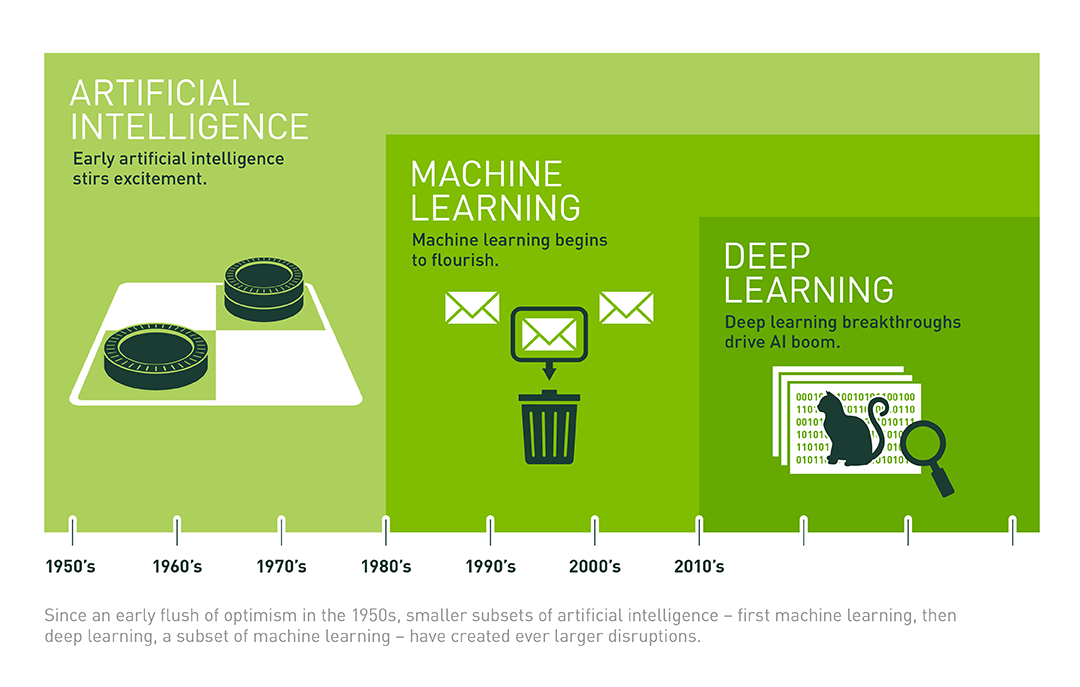
\includegraphics[scale=1.6]{AI_ML_DEEP.png}
\end{center}
\caption{Mối liên hệ AI - ML - Deep Learning}
\end{figure}

\subsection{Mạng nơ-ron sâu (Deep Neural Networks)}
\begin{figure}[!h]
\begin{center}
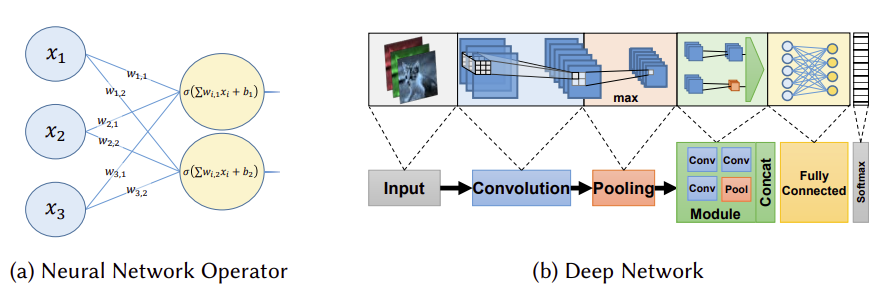
\includegraphics[scale=0.8]{DNN.PNG}
\end{center}
\caption{Kiến trúc Mạng nơ-ron sâu}
\end{figure}

\subsubsection{Nơ-ron}
Thành phần cơ bản của một mạng nơ-ron là nơ-ron. Nó được mô phỏng theo bộ não, một tế bào thần kinh nhân tạo (hình 1.2.1 a) tích lũy tín hiệu từ các tế bào thần kinh khác được kết nối bởi các khớp thần kinh. Một hàm kích hoạt được áp dụng trên giá trị tích lũy, làm tăng thêm tính phi tuyến tính cho mạng và xác định tín hiệu mà nơ-ron này “bắn” đến các vùng lân cận của nó.

\subsubsection{Mạng nơ ron}
Mạng được tạo nên từ các tầng (layer), mỗi tầng có một lượng lớn nút (node), các nút của tầng này kết nối với các nút của tầng trước đó thông qua các liên kết, mỗi liên kết có một trọng số (weight) và mỗi tầng có một hệ số tự do (bias)\\

Việc học của mạng nơ-ron nhân tạo chính là việc điều chỉnh các trọng số sao cho được bộ hệ số phù hợp nhất. 
\begin{figure}[!ht]
\begin{center}
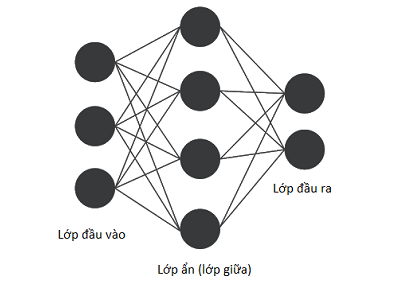
\includegraphics[scale=0.9]{ANN.png}
\end{center}
\caption{Mạng nơ-ron nhân tạo có 1 lớp ẩn}
\end{figure}

Mạng nơ-ron bao gồm 03 lớp chính là:
\begin{itemize}
	\item \textbf{Lớp đầu vào} (Input layer): là lớp nằm tận cùng bên trái, thể hiện các đầu vào của mạng;
	\item \textbf{Lớp đầu ra} (Output layer): là lớp nằm tận cùng bên phải, thể lớp đầu ra của mạng;
	\item \textbf{Lớp ẩn} (Hidden layer): là những lớp nằm giữa lớp vào và lớp ra, thể hiện suy luận của mạng.
\end{itemize}
Một mạng nơ-ron chỉ có một lớp đầu vào, một lớp đầu ra nhưng có thể không có hoặc có rất nhiều lớp ẩn.

\subsection{Các yếu tố trong huấn luyện một mô hình Mạng Nơ-ron}
\begin{enumerate}[-]
\item \textbf{Dữ liệu:} Để có một mô hình tốt thì yếu tố \underline{quan trọng nhất} là dữ liệu. Trong xã hội với sự phát triển mạnh mẽ của công nghệ thông tin như hiện nay thì việc thu thập dữ liệu không còn quá khó khăn.  Cũng bởi vậy mà thuật ngữ "Dữ liệu lớn"  hiện nay đang đang được nhắc đến như nền tảng của cuộc các mạng 4.0.\\
Tập dữ liệu được gọi là "dữ liệu lớn" nếu có 04 đặc trưng sau:
\begin{itemize}
	\item Dung lượng: kích thước của dữ liệu xác định giá trị và tiềm năng của dữ liệu có được coi là lớn không.
	\item Tính đa dạng: dữ liệu được thu thập từ nhiều nguồn và có nhiều kiểu dữ liệu cũng như cấu trúc khác nhau.
	\item Vân tốc: tốc độ tạo ra và xử lý dữ liệu cần đáp ứng nhu cầu và đáp ứng được nhu cầu tăng trưởng.
	\item Tính xác thưc: dữ liệu cẩn đảm bảo chất lượng và tính chính xác.
\end{itemize}
Do vậy, thông thường dữ liệu cần được chuẩn bị trước và cần tiều xử lý trước khi đưa vào mô hình.

\item \textbf{Mô hình}: có rất nhiều mô hình khác nhau để giải quyết một bài toán , tuy nhiên cần lựa chọn một mô hình phù hợp với tập dữ liệu để mang lại kết quả tốt nhất.

\item \textbf{Hàm mục tiêu}: sau khi đưa dữ liệu vào, với mong muốn có được một kết quả đầu ra sát với thực tế nhất chính là nguyên nhân hàm mục tiêu ra đời. Hàm mục tiêu cho phép ước lượng độ chính xác của kết quả mô hình. Toàn bộ các bước hiệu chỉnh cách máy học là để tối ưu chức năng này.

\item \textbf{Thuật toán tối ưu}: yếu tố cuối cùng là thuật toán để tối ưu mô hình. Thông qua thuật toán này, chúng ta thay đổi các tham số để tối ưu hóa hàm mục tiêu.

\end{enumerate}

\begin{figure}[!h]
\begin{center}
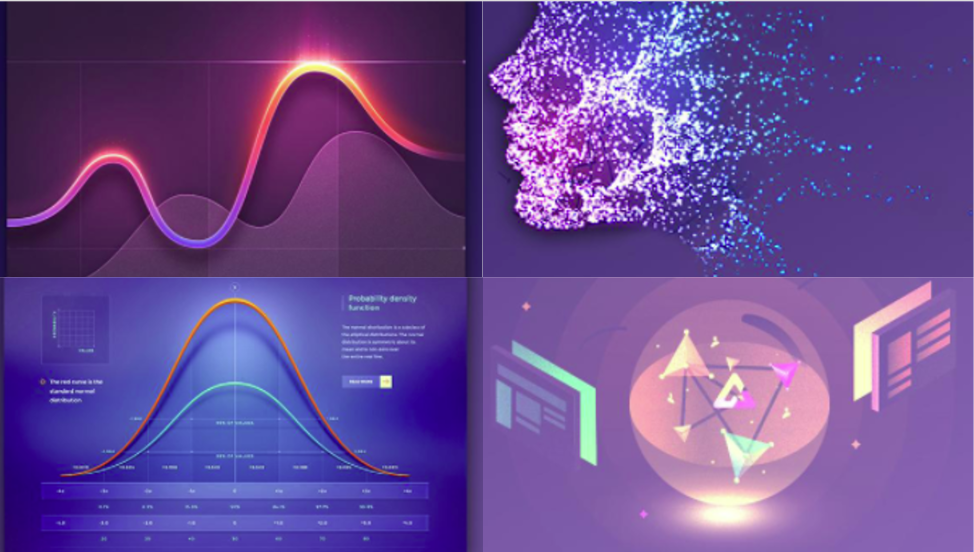
\includegraphics[scale=0.7]{Deep_save.png}
\end{center}
\caption{Các yếu tố trong Deep Learning}
\end{figure}
%%============================
\newpage
\section{Kiến trúc máy tính song song}
Phần này là tổng quan ngắn gọn về kiến trúc song song được sử dụng để thực hiện các vấn đề học tập trong thực tế. Chúng có thể được phân loại một cách khái quát thành hệ thống một máy (thường là bộ nhớ dùng chung) và nhiều máy (thường là bộ nhớ phân tán).

\subsection{Máy tính song song đơn (Single-machine Parallelism)}
Song song là phổ biến trong kiến trúc máy tính ngày nay, bên trong chip ở dạng kết nối và thực thi không theo thứ tự cũng như tiếp xúc với lập trình viê ở dạng hệ thống đa lõi (multi-core) hoặc nhiều giao tiếp (multi-socket).\\

Hệ thống đa lõi đã sinh ra từ khá lâu và được lập trình với một trong ba cách:
\begin{enumerate}[-]
	\item Đa tiến trình (multiple processes): phân phối dữ liệu là mối quan tâm hàng đầu của lập trình viên;
	\item Đa luồng (multiple threads): lập trình viên chỉ quan tâm đến tính song song, để dữ liệu xáo trộn vào hệ thống phần cứng.
	\item Kết hợp cả hai;
\end{enumerate}

\begin{figure}[!h]
\begin{center}
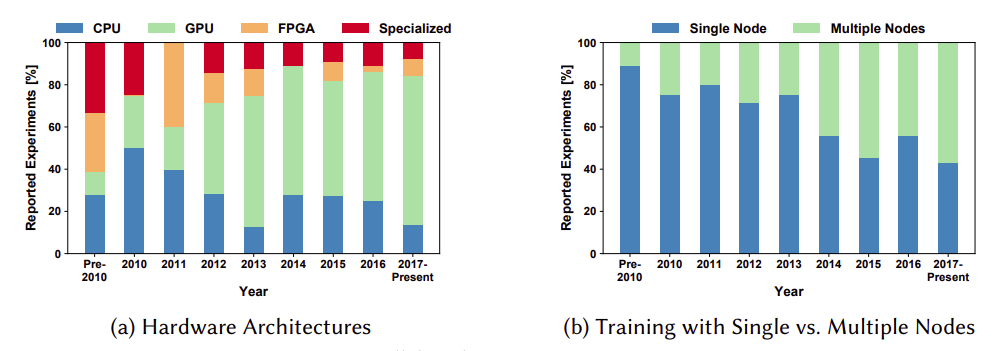
\includegraphics[scale=0.75]{parallel_Deep.PNG}
\end{center}
\caption{Kiến trúc song song trong Học sâu}
\end{figure}

Các CPU có mục đích chung đã được tối ưu hóa các khối lượng công việc chung , từ các ứng dụng máy tính để bàn theo hướng sự kiện đến các tác vụ máy chủ trung tâm dữ liệu. Trong khi các tác vụ máy học thường được tính toán chuyên sâu, khiến CPU tỏ ra ngày càng kém hiệu quả trong việc đào tạo các mô hình phức tạp.\\

Thay vào đó, việc đào tạo trở lên dễ dàng hơn khi đào tạo bằng bộ xử lý đồ họa (GPU) hoặc mảng cổng lập trình trường (Field-Programmable Gate Arrays - FPGA). Các thiết bị này tập trung vào thông thượng tính toán bằng cách chuyên biệt hóa kiến trúc của chúng để tận dụng tính song song cao của dữ liệu trong công việc.\\

Field-Programmable Gate Arrays  là một loại mạch tích hợp cỡ lớn dùng cấu trúc mảng phần tử logic mà người dùng có thể lập trình được. Chữ \textit{field} ở đây muốn chỉ đến khả năng tái lập trình "bên ngoài" của người sử dụng, không phụ thuộc vào dây chuyền sản xuất phức tạp của nhà máy bán dẫn.

\begin{figure}[!h]
\begin{center}
\includegraphics[scale=0.25]{FPGA.jpg}
\end{center}
\caption{Spartan XC3S400 của hãng Xilinx, có 400.000 cổng và tần số 50MHz-80Mhz (Nguồn: Wikipedia)}
\end{figure}

\subsection{Đa máy tính song song (multi-machine Parallelism)}
Đào tạo các mô hình quy mô lớn là một công việc đòi hỏi nhiều tính toán. Do đó, các máy đơn lẻ thường không có khả năng hoàn thành công việc này trong một khung thời gian mong muốn. Để tăng tốc tính toán hơn nữa, nó có thể được phân phối trên nhiều máy được kết nối bởi một mạng.

Các chỉ số quan trọng nhất cho mạng kết nối là:
\begin{enumerate}[-]
		\item Độ trễ;
		\item Băng thông;
		\item Tỉ lệ truyền tin (Message-Rate)
\end{enumerate}
Các công nghệ mạng khác nhau cung cấp hiệu suất khác nhau. Ví dụ, cả Ethernet hiện đại và InfiniBand đều cung cấp băng thông cao nhưng InfiniBand có độ trễ thấp hơn đáng kể và tốc độ tin nhắn cao hơn.\\
Các mạng kết nối HPC có mục đích đặc biệt có thể đạt được hiệu suất cao hơn ở cả ba chỉ số. Tuy nhiên, giao tiếp mạng nhìn chung vẫn chậm hơn giao tiếp nội bộ máy.\\ Điện toán hiệu năng cao (High-Performance Computing -HPC) là hệ thống hướng tới việc giải quyết một số bài toán như:
\begin{enumerate}[+]
	\item Nặng về xử lý: đòi hỏi khối lượng tính toán lớn;
	\item Nặng về bộ nhớ: đòi hỏi lượng bộ nhớ lớn;
	\item Nặng về dữ liệu: hoạt động trên một tập dữ liệu lớn;
	\item Thông lượng cao: bài toán đòi hỏi sự đồng bộ cao.
\end{enumerate}

\begin{figure}[!h]
\begin{center}
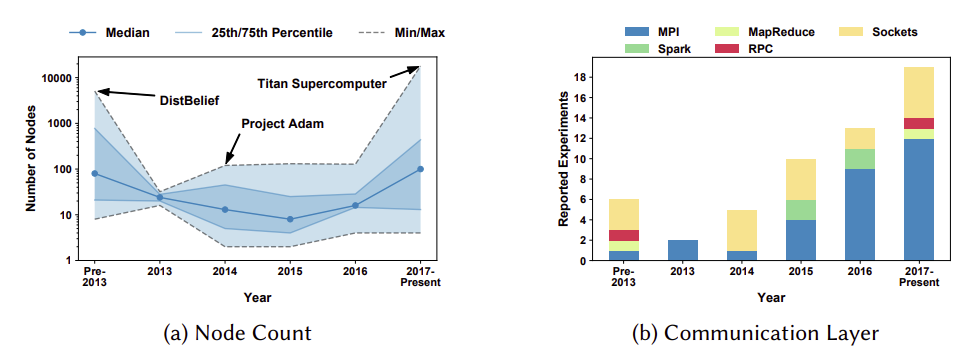
\includegraphics[scale=0.75]{parallel_Deep_2.PNG}
\end{center}
\caption{Đặc điểm của các cụm Học sâu}
\end{figure}

\subsection{Lập trình song song (Parallel Programming)}
Các kỹ thuật lập trình để thực hiện các thuật toán học song song trên các máy tính song song phụ thuộc vào kiến trúc đích. Chúng bao gồm từ triển khai theo luồng đơn giản bằng OpenMP trên các máy tính đơn lẻ.\\

Trên nhiều máy có bộ nhớ phân tán, người ta có thể sử dụng các cơ chế giao tiếp đơn giản như TCP / IP hoặc Truy cập Bộ nhớ trực tiếp từ xa (Remote Direct Memory Access - RDMA). \\

Trên các máy bộ nhớ phân tán, người ta cũng có thể sử dụng các thư viện nhằm thuận lợi hơn như Giao diện truyền thông báo (Message Passing Interface - MPI) hoặc Apache Spark.
\begin{enumerate}[-]
	\item  MPI là một thư viện cấp thấp tập trung vào việc cung cấp hiệu suất di động.
	\item Spark là một khuôn khổ cấp cao hơn tập trung nhiều hơn vào năng suất của lập trình viên.
\end{enumerate}

\subsection{Thuật toán song song (Parallel Algorithms)}
Mọi tính toán trên máy tính có thể được mô hình hóa dưới dạng đồ thị vòng có hướng (Directed Acyclic Graph - DAG). Các đỉnh của DAG là các phép tính và các cạnh là các phần phụ thuộc dữ liệu (hoặc luồng dữ liệu).\\
Sự song song tính toán trong một biểu đồ như vậy có thể được đặc trưng bởi hai tham số chính:
\begin{enumerate}[i.]
	\item Công việc của đồ thị \textbf{W	}: tổng số đỉnh của đồ thị;
	\item Độ sâu của đồ thị \textbf{D}: Số đỉnh nằm trên đường đi dài nhất của DAG.
\end{enumerate}
Hai tham số này cho phép chúng ta mô tả độ phức tạp tính toán trên một hệ thống song song.\\
Ví dụ: giả sử chúng ta có thể xử lý một thao tác trên một đơn vị thời gian thì:
\begin{enumerate}[+]
	\item Thời gian cần thiết để xử lý đồ thị trên một bộ xử lý là $T_1 = \textbf{W}$;
	\item Thời gian cần thiết để xử lý đồ thị trên vô số quá trình là $T_\infty = \textbf{D}$;
	\item Độ song song trung bình trong tính toán là $\textbf{W/D}$, thường là một số quá trình tốt để thực hiện với đồ thị;
	\item Hơn nữa, chúng tôi có thể chỉ ra rằng thời gian thực thi của một DAG như vậy trên \textit{p} bộ xử lý bị giới hạn bởi: $min\{\textbf{W}/p,\textbf{D} \leqslant T_p \leqslant \textbf{O(W}/p+\textbf{D)}\} $.
\end{enumerate}
Để rút gọn, ta áp dụng một loạt toán tử nhị phân $\oplus$ để kết hợp n giá trị thành một giá trị duy nhất.

\begin{figure}[!h]
\begin{center}
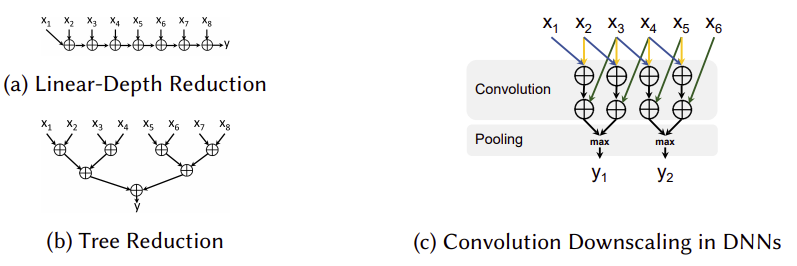
\includegraphics[scale=0.8]{parallel_Deep_3.PNG}
\end{center}
\caption{Các cách thức giảm chiều}
\end{figure}

\newpage
%%=================
\section{Tìm hiểu về Hệ thống học sâu phân tán}
\subsection{Định nghĩa}
\textbf{Hệ thống học sâu phân tán (Distributed Deep Learning Systems - DDLS)} là hệ thống đào tạo các mô hình mạng nơ-ron bằng cách sử dụng tài nguyên phân tán của một cộng đồng.\\

\begin{figure}[!h]
\begin{center}
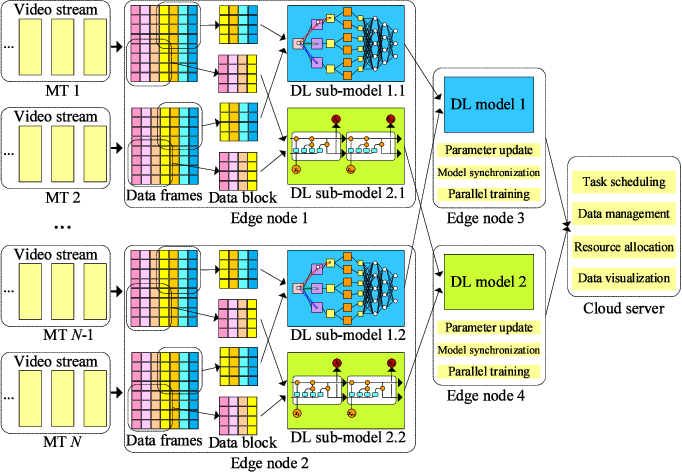
\includegraphics[scale=0.6]{DDLS.png}
\end{center}
\caption{Một mô hình DDLS}
\end{figure}

\subsection{Những vấn đề khi phát triển một hệ thống học sâu phân tán}
\begin{enumerate}[i. ]
	\item \textbf{Tính nhất quán}:  Làm thế nào chúng ta có thể đảm bảo sự đồng thuận của nhiều nút nếu chúng đồng thời hoạt động hướng tới một mục tiêu?
	
	\item \textbf{Khả năng chịu lỗi}: Nếu chúng ta phân phối khối lượng công việc của mình cho một cụm 10.000 nút tính toán, điều gì sẽ xảy ra nếu một trong số 10.000 nút bị lỗi? Có cách nào để khắc phục nó ngoài việc khởi động lại công việc ngay từ đầu không?
	
		\item \textbf{Khả năng giao tiếp}: học sâu liên quan rất nhiều đến quá trình đọc và ghi dữ liệu cũng như các thủ tục xử lý dữ liệu, thiết kế các hệ thống lưu trữ dữ liệu phù hợp với các loại môi trường khác nhau (ví dụ: hệ thống file phân tán, CPU I/O, GPU I/O,...).
		
		\item \textbf{Quản lý tài nguyên:} việc đầu tư một hệ thống máy tính với cấu hình cao là rất tốn kém. Do vậy, giải pháp là tạo một cụm máy tính được chia sẻ bởi nhiều người dùng.  Vấn đề đặt ra là làm thế nào để chúng ta có thể phân bố, quản lý tài nguyên một các hợp lý để đáp ứng được nhu cầu của mọi người mà vẫn tối ưu hóa được tài nguyên.
		
		\item \textbf{Mô hình lập trình}: chúng ta có nên lập trình các mô hình học sâu phân tán giống như các chúng ta làm đối với các mô hình không phân tán không? Có nên thiết kế một mô hình mới yêu cầu ít mã hóa hơn và cải thiện hiệu quả không?...
\end{enumerate}

Đây là những vấn đề mang tính then chốt khi muốn xây dựng mộ hệ thống học sâu phân tán. Và việc giải quyết những vấn đề này sẽ mang đến cho chúng ta những mô hình DDLS khác nhau.\\




\subsection{Các chiến lược song song}
\begin{figure}[!h]
\begin{center}
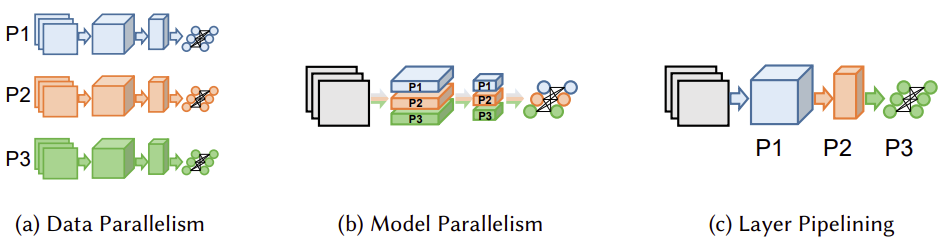
\includegraphics[scale=0.7]{parallel_1.png}
\end{center}
\caption{Lược đồ song song của mạng nơ-ron }
\end{figure}
\subsubsection{Song song dữ liệu (Data Parallelism)}
 Đây là một kỹ thuật song song hoạt động trên cơ sở phân vùng dữ liệu. \\
 
	Trong tính toán phân tán song song:
	\begin{itemize}
		\item \underline{Bước 1}: Chia dữ liệu thành một số phân vùng, với số phân vùng bằng số lượng nút tính toán.
		\item \underline{Bước 2}: Mỗi nút tính toán đóng vai trò như một công nhân sở hữu một phân vùng độc lập và mỗi công nhân thực hiện tính toán trên phân vùng của chính họ.
	\end{itemize}
	Vì có nhiều nút cùng quét dữ liệu song song nên chúng ta có thể quét nhiều dữ liệu hơn so với khi sử dụng một nút duy nhất.\\
	
	Trong học sâu phân tán, thực hiện mục tiêu tăng độ hội tụ của đào tạo mô hình bằng cách sử dụng nhiều nút trong song song dữ liệu là khá trực quan vì:
	\begin{itemize}
		\item Mỗi nút thực hiện tính toán trên phân vùng của chính nó: giảm độ dốc ngẫu nhiên.
		\item Tạo ra một tập hợp các thông số mới trên đó.
		\item Thông qua cơ chế đồng bộ với giao tiếp mạng nhằm đồng bộ tham số trên tất cả các nút.
		\item Về cơ bản, nếu quá trình đồng bộ không mất quá nhiều thời gian và cải thiện kết quả so với kết quả khi sử dụng một nút thì chúng ta đã đạt được mục tiêu của mình.
	\end{itemize}


Có hai cách tiếp cận với kiến trúc này là Máy chủ tham số không đồng bộ (Async Parameter Server) và  Kiến trúc đồng bộ hóa giảm tất cả(Sync Allreduce Architecture)\\

\textbf{Máy chủ tham số không đồng bộ}:
Công nhân thực hiện phần lớn tính toán. Mỗi công nhân nạp các tham số từ máy chủ tham số, sau khi tính toán song nó gửi các gradient qua trở lại máy chủ tham số. Sau đó máy chủ sẽ tổng hợp những gradient này một cách độc lập. 

\begin{figure}[!h]
\begin{center}
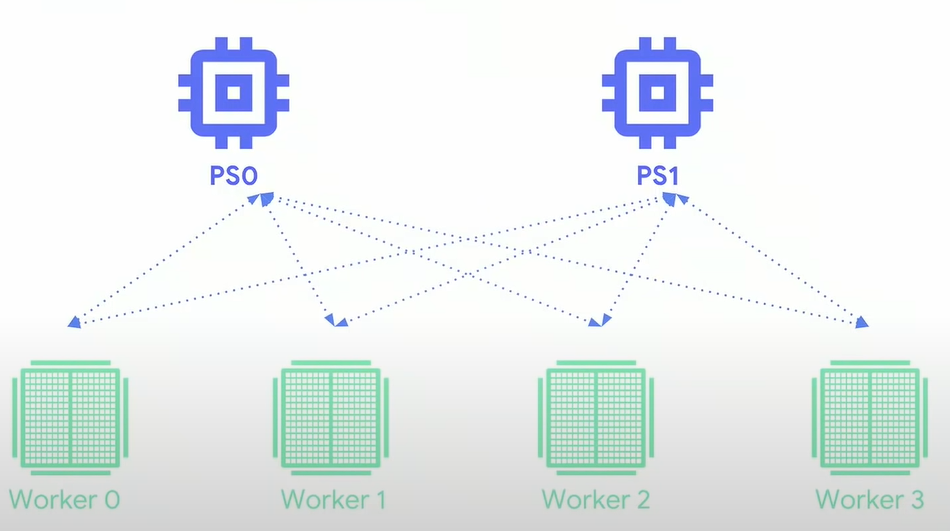
\includegraphics[scale=0.5]{Async.PNG}
\end{center}
\caption{Máy chủ tham số không đồng bộ}
\end{figure}

\begin{itemize}
	\item Ưu điểm:
	\begin{enumerate}[-]
		\item Cho phép chúng ta mở rộng quy mô tiếp cận cho một số lượng lớn công nhân.
		\item Vai trò của mỗi công nhân là khác nhau, ngoài ra các công nhân có thể gặp lỗi, bào trì. Điều này không ảnh hưởng đến quá trình đào tạo.
	\end{enumerate}
	\item Nhược điểm: các công nhân có thể mất tính đồng bộ tính toán của các gradient của họ trên các giá trị tham số, điều đó có thể làm trì hoãn sự hội tụ.
\end{itemize}

\textbf{Kiến trúc đồng bộ hóa giảm tất cả}: cách tiếp cận này trở nên phổ biến hơn với sự tăng tốc nhanh chóng của các bộ xử lý như sử dụng GPU. Trong cách tiếp cận này, mỗi công nhân có một bản sao các thông số của riêng nó, không có máy chủ tham số. Đặc biệt, mỗi công nhân giảm gradient dựa trên một tập con các mẫu đào tạo. Sau khi gradient được tính toán, công nhân giao tiếp với nhau để truyền các gradient và cập nhật. Thông số mô hình của tất cả công nhân đồng bộ hóa có nghĩa là quá trình tính toán tiếp theo không bắt đầu cho tới khi tất cả công nhân đều nhân được cập nhật.
\begin{itemize}
	\item Ưu điểm: giảm chi phí để các tham số hội tụ;
\end{itemize}
\begin{figure}[!h]
\begin{center}
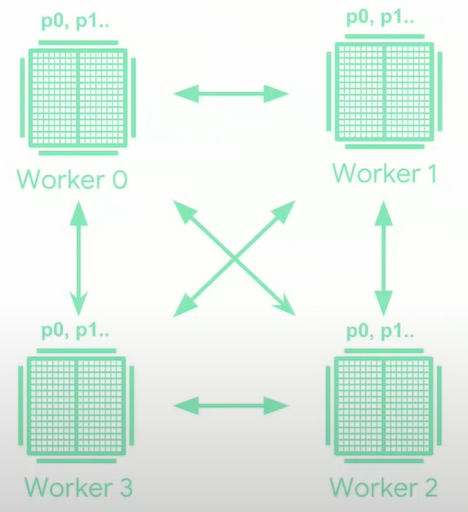
\includegraphics[scale=0.7]{sync.PNG}
\end{center}
\caption{Kiến trúc đồng bộ hóa giảm tất cả}
\end{figure}


\subsubsection{Song song mô hình (Model Parallelism)}
So với song song dữ liệu, song song mô hình là mộ khái niệm phức tạp và mơ hồ hơn nhiều. Nói chung, thay vì phân vùng dữ liệu như song song dữ liệu, chúng tôi cố gắng phân vùng chính mô hình học sâu để phân phối khối lượng công việc cho nhiều nút (công nhân) tính toán.\\
	
	Ví dụ: để nhân tử hóa một ma trận có kích thước lớn chúng ta có thể phân vùng ma trận thành các ma trận con, sau đó mỗi nút (công nhân) đảm nhận một vài khối.\\
	
	Bằng cách này, chúng ta có thể tận dụng được RAM bổ sung của nhiều nút nếu RAM trên một nít không đủ để lưu trữ tất cả các tham số trong ma trận.\\


\textit{Như vậy}, song song dữ liệu khá hiệu quả khi khích thước dữ liệu huấn luyện lớn vì chúng ta có thể quét dữ liệ nhanh hơn nhờ các nút bổ sung.\\

Song song mô hình được áp dụng  cho trường hợp kích thước của mô hình quá lớn đối với một nút, vì nó cho phép chúng ta phân vùng mô hình và tận dụng bộ nhớ bổ sung trên nhiều nút.\\

\textit{Tuy nhiên}, do chi phí gây ra bởi các tác vụ đồng bộ cũng như quá trình xử lý tại các nút mạng khiến cho thời gian để hoàn thành một vòng lặp đào tạo trên một cụm máy tính phân tán là lâu hơn so với trên một nút đơn lẻ. Do vậy, cần dành thêm thời gian để đồng bộ hóa qua nhiều nút khi kết thúc quá trình tính toán nhằm đảm bảo sự hội tụ của quá quá trình huấn luyện. parallel.

\subsubsection{Kỹ thuật đường ống (Pipelining)}
Trong học sâu, pipelining có thể đề cập đến các phép tính chồng chéo, tức là giữa lớp này và lớp tiếp theo; hoặc phân vùng DNN theo độ sâu, gán các lớp cho các bộ xử lý cụ thể.\\

Pipelining có thể được xem như một dạng song song dữ liệu, vì các phần tử (mẫu) được xử lý song song qua mạng, nhưng cũng như song song mô hình, vì chiều dài của đường ống được xác định bởi cấu trúc DNN.\\

Như vậy, mạng nơ-ron có thể được thiết kế dựa trên nguyên tắc tính toán các lớp chồng lên nhau, như trường hợp của Mạng xếp chồng sầu (Deep Stacking Networks - DSN). Trong DSN, mỗi bước tính một lớp dữ liệu được kết nối đầy đủ khác nhau. Tuy nhiên, kết quả của tất cả các bước trước đó được nối với các đầu vào của lớp.  Điều này cho phép mỗi lớp được tính toán song song một phần, do các phụ thuộc vào dữ liệu.

\begin{figure}[!h]
\begin{center}
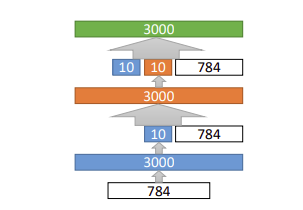
\includegraphics[scale=1.2]{DSN.PNG}
\end{center}
\caption{Mạng xếp chồng sầu (Deep Stacking Networks)}
\end{figure}


\newpage
%%=============
\section{Các thuật toán tối ưu hóa phân tán}
Theo thời gian, quy mô các mô hình cần đào tạo càng lớn. Khi đó, để đào tạo mô hình với một khoảng thời gian hợp lý thì chúng ta cần phải tính toán song song không chỉ trong một phiên bản mô hình mà cần phải phân phối trong nhiều phiên bàn của mô hình.\\

Bài tiểu luận này sẽ trình bày về so sánh hai quy trình tối ưu hóa phân tán quy mô lớn là Downpour SGD - một phương pháp trực tuyến và Sandblaster L-BFGS - một phương pháp đồng loạt.

\begin{figure}[!h]
\begin{center}
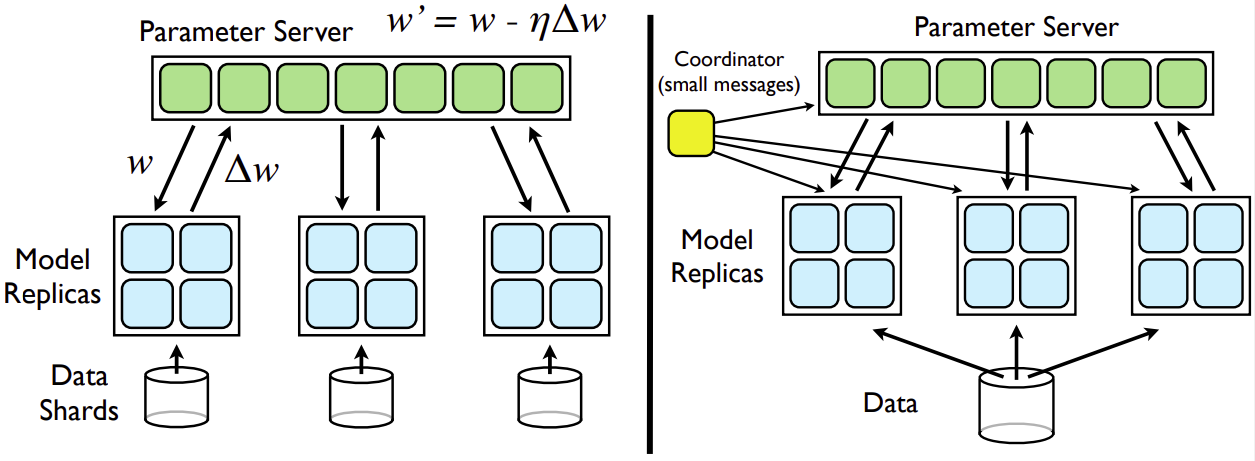
\includegraphics[scale=0.5]{SGD.PNG}
\end{center}
\caption{Trái: Downpour SGD. Bản sao mô hình tìm nạp không đồng bộ các tham số w và đẩy gradient $\bigtriangleup w$ đến máy chủ tham số. Phải:  Sandblaster L-BFGS. Một "điều phối viên" gửi các thông báo nhỏ đến các bản sao và máy chủ tham số để sắp xếp tối hư hóa hàng loạt.   }
\end{figure}


\subsection{Downpour SGD}
Stochastic gradient descent (SGD) được cho là quy trình tối ưu hóa được sử dụng phổ biến nhất để đào tạo mạng nơron học sâu. Tuy nhiên, công thức truyền thống của SGD vốn có tính tuần tự, khiến việc áp dụng cho các tập dữ liệu rất lớn là không thực tế vì thời gian cần thiết để di chuyển qua dữ liệu theo kiểu nối tiếp hoàn toàn là không thực tế.\\

Để áp dụng SGD cho các tập dữ liệu lớn, chúng ta sử dụng Downpour SGD, một biến thể của gradient ngẫu nhiên không đồng bộ. Cách tiếp cận cơ bản như sau: Chúng ta chia dữ liệu huấn luyện thành một số tập con và chạy một bản sao của mô hình trên mỗi tập con này. Các mô hình giao tiếp các bản cập nhật thông qua một máy chủ tập trung, giữ trạng thái hiện tại của tất cả các tham số cho mô hình, được phân đoạn trên nhiều máy.\\
Ví dụ: nếu chúng ta có 10 phân đoạn trên máy chủ, mỗi phân đoạn có trách nhiệm lưu trữ và áp dụng các bản cập nhật cho 1/10 số tham số của mô hình (Hình 4.0.1).\\

Cách tiếp cận này không đồng bộ theo hai khía cạnh:
\begin{enumerate}[i.]
	\item Các bản sao mô hình chạy độc lập với nhau;
	\item Các phân đoạn máy chủ tham số cũng chạy độc lập với nhau.
\end{enumerate}

Trong cách triển khai đơin giản nhất, trước khi xử lý từng lô nhỏ, một bản sao mô hình yêu cầu máy chủ tham số cung cấp bản sao cập nhật của tất cả tham số của mô hình đó.\\

Ngoài ra, có thể giảm chi phí giao tiếp của Downpour SGD bằng cách giới hạn mỗi bản sao mô hình chỉ yêu cầu các tham số cập nhật sau mỗi $n_{fetch}$ và chỉ gửi các giá trị gradient cập nhật sau mỗi bước $n_{push}$ (trong đó $n_{fetch}$ có thể không bằng $n_{push}$). Trên thực tế, quá trình tìm nạp các tham số, đẩy gradient và xử lý dữ liệu đào tạo có thể được thực hiện trong ba luồng chỉ được đồng bộ hóa yếu.\\

Đối với SGD đồng bộ, nếu hỏng một máy thì toàn bộ quá trình đào tạo bị đình trệ; trong khi đối với SGD không đồng bộ, nếu một máy trong bản sao mô hình bị lỗi, các bản sao mô hình khác tiếp tục xử lý dữ liệu huấn luyện của chúng và cập nhật các tham số mô hình thông qua máy chủ tham số. Mặt khác, nhiều hình thức xử lý không đồng bộ trong Downpour SGD thể hiện rất nhiều tính ngẫu nhiên bổ sung trong quy trình tối ưu hóa. Rõ ràng, một bản sao mô hình gần như chắc chắn đang tính toán gradient của nó dựa trên một tập hợp các tham số có thể cũ, trong đó một số bản sao mô hình khác có thể sẽ cập nhật các thông số trên máy chủ tham số trong thời gian chờ đợi. Nhưng có một số nguồn ngẫu nhiên khác ngoài điều này:
\begin{enumerate}[-]
	\item Các phân đoạn máy chủ tham số hoạt động độc lập, không có gì đảm bảo rằng tại bất kỳ thời điểm cụ thể nào, các tham số trên mỗi phân đoạn của máy chủ tham số đã trải qua cùng một số lượng cập nhật hoặc các bản cập nhật được áp dụng theo cùng một thứ tự;
	\item Hơn nữa, vì các bản sao mô hình được phép tìm nạp các tham số và đẩy gradient vào các luồng riêng biệt, do đó có thể có thêm sự mâu thuẫn nhỏ trong dấu thời gian của các tham số.
\end{enumerate}
Có rất ít cơ sở lý thuyết cho sự an toàn của các hoạt động này đối với các vấn đề không lồi, nhưng trong thực tế, chúng ta nhận thấy các yêu cầu về tính nhất quán giãn ra có hiệu quả rõ rệt.\\

Một kỹ thuật mà chúng tôi đã tìm ra để tăng đáng kể mức độ mạnh mẽ của Downpour SGD là sử dụng quy trình tỷ lệ học tập thích ứng Adagrad. Thay vì sử dụng một tốc độ học cố định duy nhất trên máy chủ tham số ($\eta$ trong Hình 4.0.1), Adagrad sử dụng một tốc độ học thích ứng riêng cho từng tham số.\\

Gọi $\eta_{i,K}$ là tốc độ học của tham số thứ i tại lần lặp K và $w_{i,K}$ là gradient của nó, sau đó đặt: $\eta_{i,K} = \gamma / \sqrt{\sum_{j=1}^K \Delta w_{i,j}^2}$. Bởi vì các tỷ lệ học tập này chỉ được tính từ các gradient bình phương tổng hợp của mỗi thông số, Adagrad dễ dàng được triển khai cục bộ trong mỗi phân đoạn máy chủ thông số. Giá trị của $\gamma$, hệ số tỷ lệ không đổi cho tất cả các tỷ lệ học tập, thường lớn hơn so với tỷ lệ học tập cố định tốt nhất được sử dụng mà không có Adagrad.\\

Việc sử dụng Adagrad mở rộng số lượng tối đa các bản sao mô hình có thể hoạt động hiệu quả đồng thời và kết hợp với thực hành đào tạo mô hình “khởi động sớm” chỉ với một bản sao mô hình duy nhất trước khi giải phóng các bản sao khác, nó hầu như đã loại bỏ những lo ngại về tính ổn định trong việc đào tạo mạng sâu bằng cách sử dụng Downpour SGD.

\subsection{Sandblaster L-BFGS}
Phương pháp lô đã được chứng minh và thực nghiệm là hoạt động tốt trong việc đào tạo các mạng sâu nhỏ. Để áp dụng các phương pháp này cho các mô hình lớn và bộ dữ liệu lớn, chúng ta sử dụng  khung tối ưu hóa hàng loạt Sandblaster và xem xét về việc triển khai L-BFGS bằng cách sử dụng khung này.\\

Một ý tưởng chính trong Sandblaster là lưu trữ và thao tác với tham số phân tán. Cốt lõi của thuật toán tối ưu hóa nằm trong quy trình điều phối viên (Hình 4.0.1), quy trình này không có quyền truy cập trực tiếp vào các tham số mô hình. Thay vào đó, điều phối viên đưa ra các lệnh rút ra từ một tập hợp nhỏ các hoạt động (ví dụ: tích chấp, chia tỷ lệ, phép cộng theo hệ số, phép nhân) có thể được thực hiện bởi từng phân đoạn máy chủ tham số một cách độc lập, với kết quả được lưu trữ cục bộ trên cùng một phân đoạn. Điều này cho phép chạy các mô hình lớn (hàng tỷ tham số) mà không phải chịu phí gửi tất cả các tham số và gradient đến một máy chủ trung tâm duy nhất.\\

Trong các triển khai song song điển hình của L-BFGS, dữ liệu được phân phối cho nhiều máy và mỗi máy chịu trách nhiệm tính toán gradient trên một tập hợp con cụ thể của các tập dữ liệu. Các gradient được gửi trở lại máy chủ trung tâm (hoặc tổng hợp qua một cây). 
Do vậy, không mở rộng quy mô tốt cho các mô hình lớn. Để giải quyết vấn đề này, chúng ta sử dụng sơ đồ cân bằng tải sau. Người điều phối chỉ định một trong số N bản sao mô hình để phần nhỏ công việc, nhỏ hơn nhiều so với 1 / N tổng kích thước của một lô, và chỉ định bản sao mô hình các phần mới bất cứ khi nào chúng rảnh. Với cách tiếp cận này, các bản sao mô hình nhanh hơn sẽ làm được nhiều việc hơn các bản sao chậm hơn. Để quản lý thêm các bản sao mô hình chậm vào cuối một lô, điều phối viên lập lịch cho nhiều bản sao của các phần còn tồn đọng và sử dụng kết quả từ bất kỳ bản sao mô hình nào hoàn thành trước.\\

Tìm nạp trước dữ liệu, cùng với việc hỗ trợ mối quan hệ dữ liệu bằng cách gán  phần dữ liệu tuần tự cho cùng một nhân viên làm cho việc truy cập dữ liệu trở nên không thành vấn đề. Ngược lại với Downpour SGD, đòi hỏi tần số tương đối cao, đồng bộ hóa tham số băng thông lớn với máy chủ tham số, Sandblaster chỉ tìm nạp các tham số vào đầu mỗi đợt (khi chúng đã được điều phối viên cập nhật) và chỉ gửi các gradient sau mỗi vài phần đã hoàn thành (để bảo vệ khỏi lỗi sao chép và khởi động lại).

%%==============================================
\newpage
\section{Tìm hiểu về Đào tạo TensorFlow phân tán (Distributed TensorFlow training) }

\subsection{TensorFlow là gì?}
TensorFlow là một thư viện phần mềm mã nguồn mở dành cho máy học trong nhiều loại hình tác vụ nhận thức và hiểu ngôn ngữ. TensorFlow do đội ngũ kỹ sư của  Google Brain xây dụng và là thế hệ thứ hai của hệ thống máy học (trước đó là DistBelief). Các thư viện của TensorFlow sinh ra nhằm mục đích huấn luyện các bài toán mạng nơ-ron.

\subsection{TensorFlow API}
Là sơ đồ của công cụ thực thi phân tán của TensorFlow. TensorFlow được viết bằng ngôn ngữ C ++, nhưng giao diện người dùng được thực hiện bằng cách sử dụng các ngôn ngữ khác nhau như C, C ++, R, Java,..\\

Python là ngôn ngữ dễ nhận biết nhất và là ngôn ngữ "chính" khi nói đến TensorFlow và sự phát triển của nó. API Python về bản chất rất đa dạng nên chọn cấp độ API nào trong TensorFlow sao cho phù hợp với công việc.\\

Các chức năng có sẵn của TensorFlow API như:
\begin{enumerate}[-]
	\item Tự động checkpoint;
	\item Tự động ghi nhật ký;
	\item Đào tạo / đánh giá / dự đoán riêng biệt;
	\item Phân phối đào tạo đơn giản hóa.
\end{enumerate}

\lstset{language=Python}
\lstset{frame=lines}
\lstset{caption={Đào tạo trên một GPU với Distribution Strategy}}
\lstset{label={lst:code_direct}}
\lstset{basicstyle=\footnotesize}
\begin{lstlisting}
classifier = tf.estimator.Estimator(
	model_fn=model_function,
	model_dir=model_dir,
	condig=run_config)
	
classidier.train(input_fn=input_function)
\end{lstlisting}

TensorFlow hỗ trợ chuyển từ đào tạo đơn GPU sang đào tạo với nhiều GPUs một cách dễ dàng. Ví như đoạn chương trình bên trên, để có thể chạy trên nhiều GPUs, chúng ta chỉ cần bổ sung 2 dòng lệnh:

\lstset{language=Python}
\lstset{frame=lines}
\lstset{caption={Đào tạo trên nhiều GPUs với Distribution Strategy}}
\lstset{label={lst:code_direct}}
\lstset{basicstyle=\footnotesize}
\begin{lstlisting}
// MirrorredSreategy phep phan tan tren nhieu GPUs.
distribution = tf.contrib.distribute.MirrorredSreategy() 
// RunConfig xac dinh cau hinh de dao tao mo hinh.
run_config = tf.estimator.RunConfig(train_distribute=distribution) 

classifier = tf.estimator.Estimator(
	model_fn=model_function,
	model_dir=model_dir,
	condig=run_config)
	
classidier.train(input_fn=input_function)
\end{lstlisting}

\textbf{Giới thiệu một số thư viện khi phân tán với TensorFlow}

\lstset{language=Python}
\lstset{frame=lines}
\lstset{caption={API TensorFlow để phân phối đào tạo trên nhiều GPU, nhiều máy hoặc TPU}}
\lstset{label={lst:code_direct}}
\lstset{basicstyle=\footnotesize}
\begin{lstlisting}
			tf.distribute.Strategy
\end{lstlisting}
Sử dụng API này, chúng ta có thể phân phối các mô hình và mã đào tạo hiện có của mình với những sự thay đổi tối thiểu.
\lstset{language=Python}
\lstset{frame=lines}
\lstset{caption={Hỗ trợ đào tạo phân tán đồng bộ trên nhiều GPU trên một máy}}
\lstset{label={lst:code_direct}}
\lstset{basicstyle=\footnotesize}
\begin{lstlisting}
			tf.distribute.MirroredStrategy
\end{lstlisting}
Nó tạo ra một bản sao cho mỗi thiết bị GPU. Mỗi biến trong mô hình được sao chép trên tất cả các bản sao. Cùng với nhau, các biến này tạo thành một biến khái niệm duy nhất được gọi là MirroredVariable. Các biến này được giữ đồng bộ với nhau bằng cách áp dụng các bản cập nhật giống hệt nhau.

\lstset{language=Python}
\lstset{frame=lines}
\lstset{caption={Đào tạo mô hình trên các Đơn vị xử lý Tensor (TPU)}}
\lstset{label={lst:code_direct}}
\lstset{basicstyle=\footnotesize}
\begin{lstlisting}
			tf.distribute.TPUStrategy
\end{lstlisting}
TPU là ASIC chuyên dụng của Google được thiết kế để tăng tốc đáng kể khối lượng công việc học máy. Chúng có sẵn trên Google Colab, TPU Research Cloud, và Cloud TPU.Về kiến trúc đào tạo phân tán, TPUStrategy cũng giống như MirroredStrategy - nó triển khai đào tạo phân tán đồng bộ. TPU cung cấp việc triển khai hiệu quả và các hoạt động tập thể khác trên nhiều lõi TPU, được sử dụng trong TPUStrategy.

%%==============
\newpage

\section{Kết quả (trích dẫn từ một số bài báo khoa học)}

\subsection{Kết quả nghiên cứu của các Giáo sư, Chuyên gia của Google Inc }
Bài báo đã đánh giá các thuật toán tối ưu hóa của họ bằng cách áp dụng chúng vào các mô hình đào tạo cho hai vấn đề học sâu khác nhau: nhận dạng đối tượng trong ảnh tĩnh và xử lý âm thanh để nhận dạng giọng nói.\\

hiệm vụ nhận dạng giọng nói là phân loại vùng trung tâm (hoặc khung) trong một đoạn âm thanh ngắn thành một trong số hàng nghìn trạng thái âm thanh. Bài báo đã sử dụng một mạng học sâu với năm lớp: bốn lớp ẩn với các hàm kích hoạt sigmoid, ở mỗi lớp có 2560 nút và đầu ra là một hàm softmax với 8192 nút. Đầu vào là 11 khung lời nói 25 ms chồng lên nhau liên tiếp, mỗi khung được biểu diễn bằng 40 giá trị log-energy. Mạng được kết nối đầy đủ từng lớp, với tổng số khoảng 42 triệu tham số.Bài báo đã đào tạo trên một tập dữ liệu gồm 1,1 tỷ ví dụ được gắn nhãn yếu và được đánh giá trên tập thử nghiệm.\\

Để nhận dạng đối tượng trực quan, bài báo đã đào tạo một mạng nơ-ron lớn hơn với các trường tiếp nhận được kết nối cục bộ trên tập dữ liệu ImageNet gồm 16 triệu hình ảnh, mỗi hình ảnh được chia tỷ lệ thành 100x100 pixel. Mạng có ba giai đoạn, mỗi giai đoạn bao gồm \textbf{lọc}, \textbf{gộp} và \textbf{chuẩn hóa tương phản cục bộ}, trong đó mỗi nút trong lớp lọc được kết nối với một bản vá 10x10 ở lớp bên dưới. Lớp đầu ra bao gồm 21 nghìn nút phân loại hậu cần một so với tất cả, một nút cho mỗi danh mục đối tượng ImageNet.\\

Mô hình giọng nói có kích thước vừa phải chạy trên 8 máy, có tốc độ tính toán \textbf{ nhanh hơn 2,2 lần} so với sử dụng một máy duy nhất (Cấu hình của mỗi máy được cố định không lớn hơn 20 cores trên mỗi máy).

\begin{figure}[!h]
	\begin{center}
		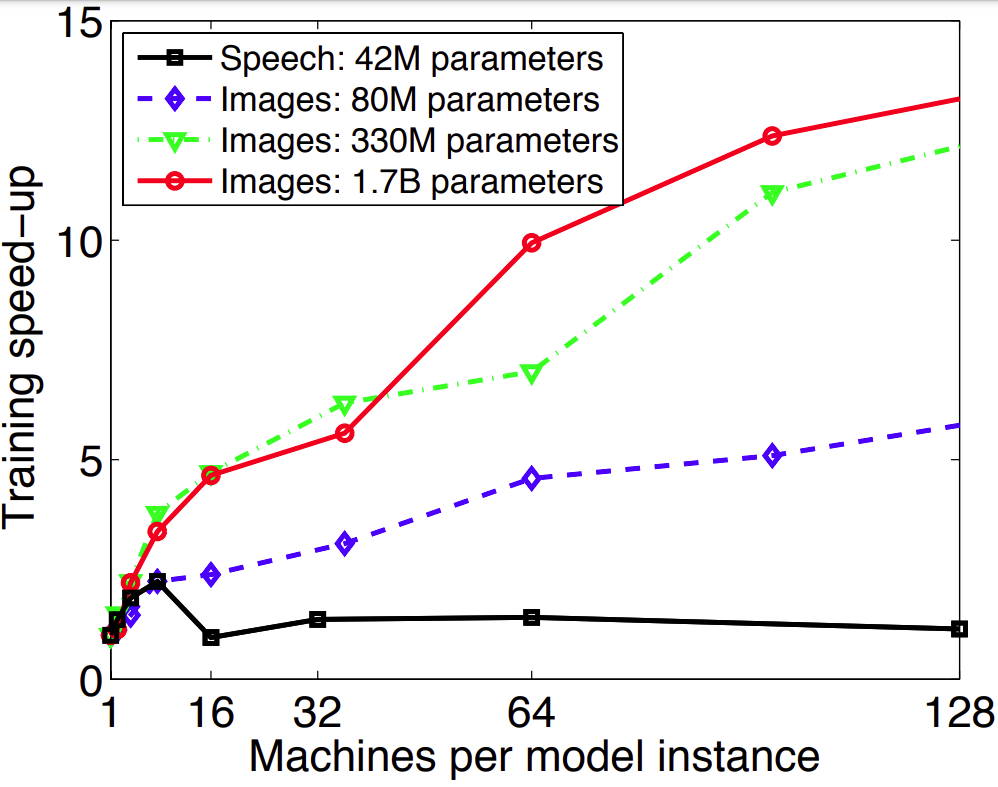
\includegraphics[scale=0.65]{GG_1.PNG}
	\end{center}
	\caption{Đào tạo tăng tốc cho bốn mạng học sâu khác nhau như một chức năng của các máy được phân bổ cho một phiên bản mô hình DistBelief duy nhất. Các mô hình có nhiều tham số được hưởng lợi nhiều hơn từ việc sử dụng các máy bổ sung so với các mô hình có ít tham số hơn}
\end{figure}

\begin{figure}[!h]
	\begin{center}
		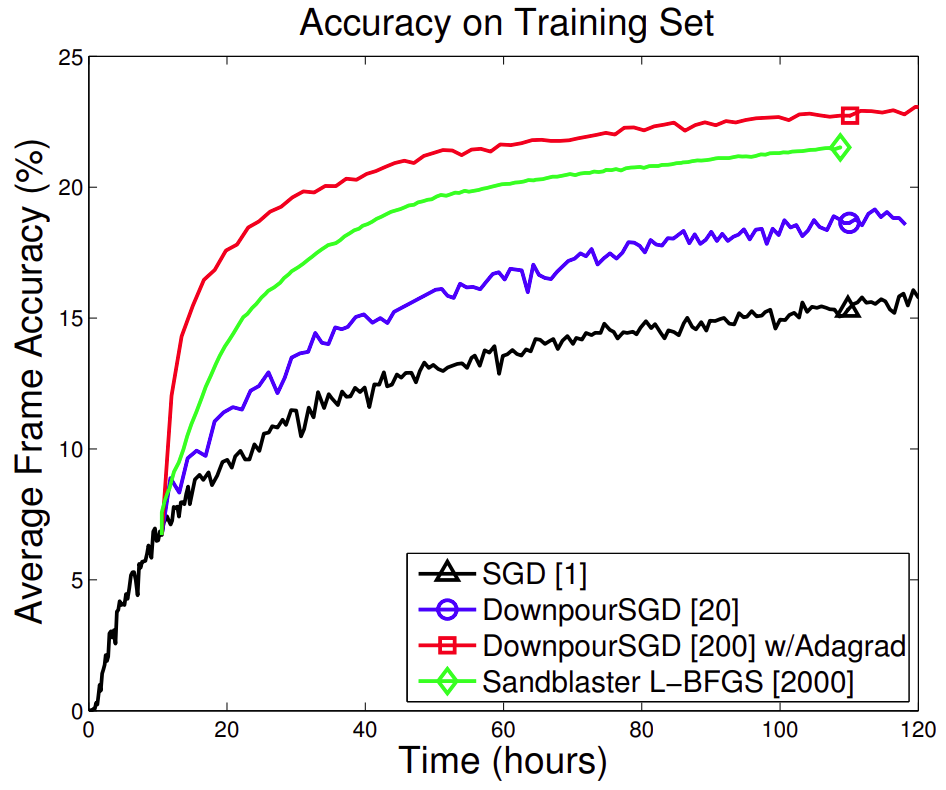
\includegraphics[scale=0.37]{GG_2.PNG}
		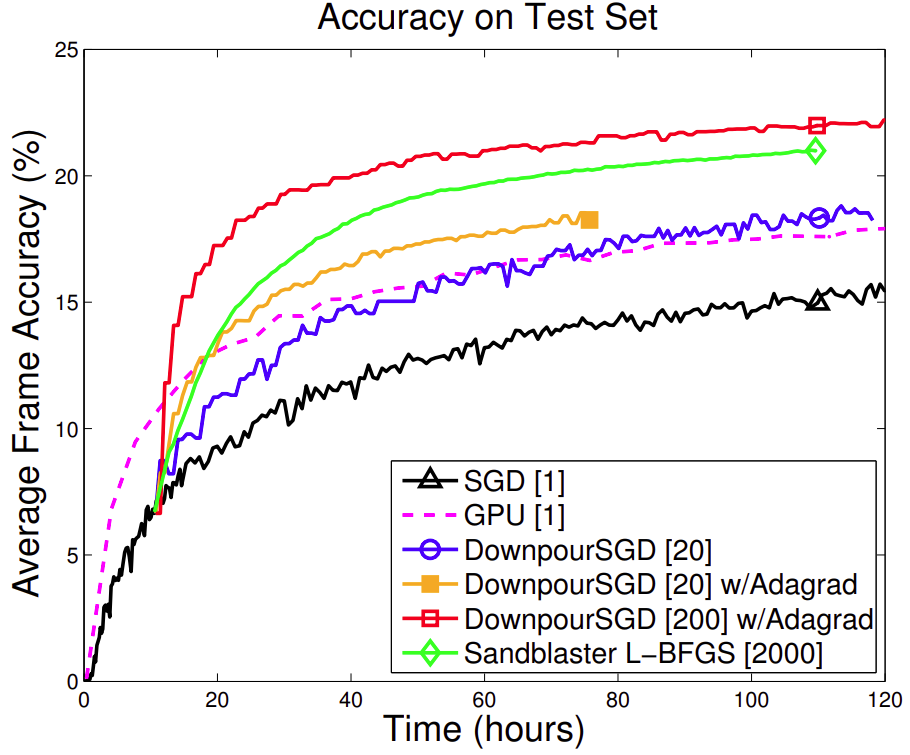
\includegraphics[scale=0.39]{GG_3.PNG}
	\end{center}
	\caption{Trái: độ chính xác đào tạo (trên một phần của tập hợp đào tạo) cho các phương pháp tối ưu hóa khác nhau. Phải:  Độ chính xác của phân loại trên tập kiểm tra. Thử nghiệm Downpour và Sandblaster được khởi chạy bằng cách sử dụng cùng một thời điểm khởi động sau SGD đơn giản khoảng 10 giờ}
\end{figure}

Việc phân vùng mô hình trên hơn 8 máy thực sự làm chậm quá trình đào tạo, vì chi phí mạng bắt đầu chiếm ưu thế trong cấu trúc mạng được kết nối đầy đủ và mỗi máy có ít công việc hơn để thực hiện với nhiều phân vùng hơn. Ngược lại, với mô hình xử lý hình ảnh kết nối cục bộ, lớn hơn nhiều có thể được hưởng lợi từ việc sử dụng nhiều máy hơn cho mỗi bản sao mô hình. Mô hình lớn nhất, với 1,7 tỷ tham số được hưởng lợi nhiều nhất, cho tốc độ nhanh hơn 12 lần khi sử dụng 81 máy. Đối với những mô hình lớn này, sử dụng nhiều máy hơn sẽ làm tiếp tục tăng tốc độ, nhưng lợi nhuận giảm dần.\\

\textbf{So sánh các phương pháp tối ưu}:  Để đánh giá các thủ tục tối ưu hóa phân tán được đề xuất, bài báo đã chạy mô hình giọng nói được mô tả ở trên với nhiều cấu hình khác nhau. Bài báo xem xét hai quy trình tối ưu hóa đường cơ sở: đào tạo mô hình DistBelief (trên 8 phân vùng) bằng SGD thông thường (bản sao đơn) và đào tạo mô hình giống hệt trên GPU bằng CUDA. Ba phương pháp tối ưu hóa phân tán được đề cập là: Downpour SGD với tỉ lệ học (learning rate) học cố định, Downpour SGD với tỉ lệ học của Adagrad và Sandblaster L-BFGS.\\

Hình 5.1.2 cho thấy hiệu suất phân loại như một hàm của thời gian huấn luyện cho mỗi phương pháp này trên cả tập huấn luyện và tập kiểm tra. Mục tiêu là \textit{ đạt được độ chính xác của bộ thử nghiệm tối đa trong khoảng thời gian đào tạo tối thiểu, bất kể yêu cầu về nguồn lực}.\\

SGD bản sao đơn (đường cong màu đen) là loại huấn luyện chậm nhất. Downpour SGD với 20 bản sao mô hình (đường cong màu xanh nước biển) cho thấy một sự cải thiện đáng kể. Downpour SGD với 20 bản sao cộng với Adagrad (đường cong màu cam) nhanh hơn một chút. Sandblaster L-BFGS sử dụng 2000 bản sao mô hình (đường cong màu xanh lá cây) lại nhanh hơn đáng kể. Tuy nhiên, nhanh nhất là Downpour SGD cộng với Adagrad với 200 bản sao mô hình (đường cong màu đỏ).\\

Như vậy, với quyền truy cập vào đủ tài nguyên CPU, cả Sandblaster L-BFGS và Downpour SGD với Adagrad đều có thể đào tạo các mô hình về cơ bản nhanh hơn đáng kể so với GPU hiệu suất cao.\\

Để xem xét hiệu suất của các phương pháp bài báo cố định  độ chính xác (16\%) và đo thời gian mỗi phương pháp đạt được độ chính xác đó với cùng lượng tài nguyên CPU. Hình 5.1.3. Một trong bốn điểm trên mỗi dấu vết tương ứng với một cấu hình đào tạo được hiển thị trong Hình 5.1.2, ba điểm còn lại là cấu hình thay thế.

\begin{figure}[!h]
	\begin{center}
		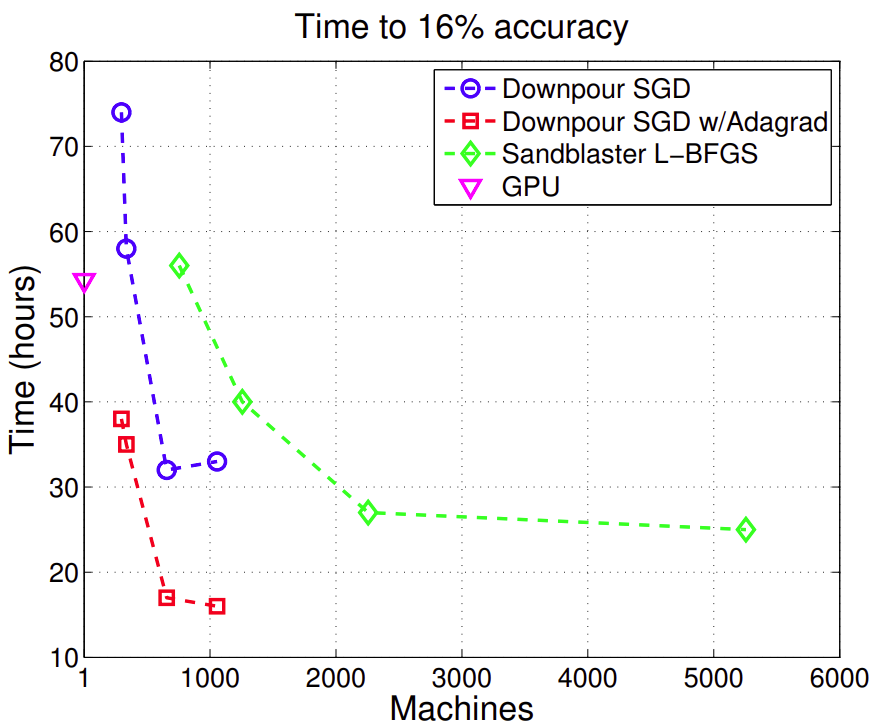
\includegraphics[scale=0.39]{GG_4.PNG}
		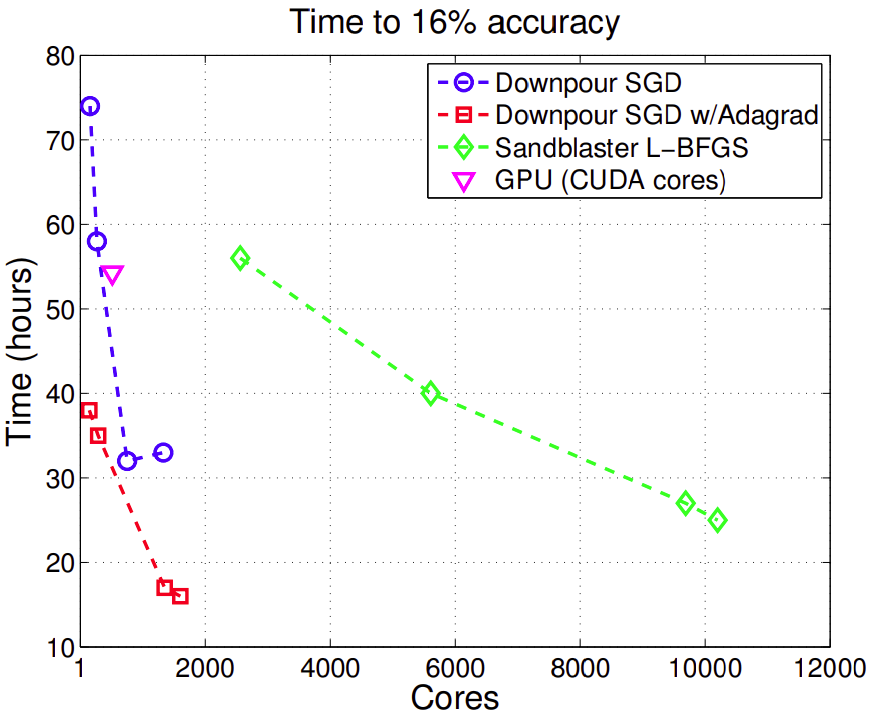
\includegraphics[scale=0.39]{GG_5.PNG}
	\end{center}
	\caption{Thời gian để đạt được độ chính xác cố định (16\%) cho các chiến lược tối ưu hóa khác nhau với số lượng máy (trái) và số lượng core (phải)}
\end{figure}

\underline{Nhận xét:} 
\begin{enumerate}[i. ]
	\item Các điểm gần nguồn gốc hơn sẽ thích hợp hơn ở chỗ chúng mất ít thời gian hơn khi sử dụng ít tài nguyên hơn. Về vấn đề này, SGD Downpour sử dụng Adagrad dường như là sự cân bằng tốt nhất: Đối với bất kỳ ngân sách máy hoặc lõi cố định nào, Downpour SGD với Adagrad mất ít thời gian hơn để đạt được mục tiêu chính xác hơn so với Downpour SGD với tốc độ học cố định hoặc Sandblaster L- BFGS;
	\item  Đối với bất kỳ thời gian đào tạo được phân bổ nào để đạt được mục tiêu chính xác, Downpour SGD với Adagrad sử dụng ít tài nguyên hơn Sandblaster L-BFGS và trong nhiều trường hợp Downpour SGD với tốc độ học cố định thậm chí không thể đạt được mục tiêu trong thời hạn;
	\item  Sandblaster L-BFGS cho thấy nhiều hứa hẹn về khả năng mở rộng quy mô với các lõi bổ sung, cho thấy rằng cuối cùng nó có thể tạo ra thời gian đào tạo nhanh nhất nếu được sử dụng với ngân sách tài nguyên cực lớn (ví dụ: 30 nghìn cores).
\end{enumerate}

\subsection{Áp dụng phương pháp đào tạo học sâu phân tán của phòng nghiên cứu MIT Lincoln}
Các nhà nghiên cứu tại phòng nghiên cứu MIT Lincoln đã sử dụng mô hình mạng nơ-ron để đưa ra dự báo về lượng mưa. Các Nhà khoa học đã sử dụng mô hình Convolutional Neural Networks (CNNs) để giải bài toán này. Đặc thù của các bài toán dự báo thời tiết là hình ảnh thời tiết đầu vào có độ phân giải cao kết hợp với độ phức tạp cần thiết của mô hình để xử lý dữ liệu khiến việc đào tào mô hình CNN rất mất thời gian.\\

Để giải quyết vấn đề này, một mô hình song song dữ liệu được triển khai trong đó mô hình CNN được sao chép trên nhiều nút máy tính và các lô đào tạo được phân phối trên nhiều nút. Bằng cách tận dụng nhiều GPUs,các nhà khoa học thấy rằng thời gian đào tạo một kiến trúc mô hình dự báo nhất định có thể \textbf{giảm từ 59 giờ xuống chỉ còn hơn 1 giờ}.\\

\textit{Thông số kỹ thuật thiết bị}: \\
Quá trình đào tạo mô hình đã được thực hiện trên siêu máy tính TX-Green của trung tâm phòng nghiên cứu siêu máy tính Lincoln. 
Đây là một hệ thống không đồng nhất bao gồm nhiều nền tảng phần cứng khác nhau của AMD, Intel và NVIDIA. Các bài kiểm tra trong bài báo này được thực hiện trên các nút máy tính có GPU NVIDIA K80. Các nút GPU trong cụm bao gồm bộ xử lý Haswell ổ cắm kép (Intel Xeon E5-2680 v4 @ 2,40GHz) và hai GPU NVIDIA K80. Mỗi GPU K80 bao gồm hai thiết bị GK210 với 11,44 GB bộ nhớ GDDR5 cho mỗi thiết bị. Do đó, một quá trình chạy trên các nút máy tính này sẽ thấy bốn thiết bị GPU.\\

\textit{A. Đào tạo trên đơn GPU}\\
Mô hình dự báo thời tiết đã được triển khai trong TensorFlow 1.12 bằng cách sử dụng API Keras. Mạng này có 17.395.992 tham số có thể huấn luyện. Tập dữ liệu được dùng là: 
\begin{enumerate}[-]
	\item Tập 1: 17.833 hình ảnh kích thước 256x256 pixel.
	\item Tập 2: 45.897 hình ảnh bảo gồm các ảnh khác và tất cả ảnh có trong tập 1.
\end{enumerate}
Trong cả 2 trường hợp, tập kiểm tra là 10.052 ảnh được sử dụng.\\

Mô hình đã được đào tạo trên cả hai tập dữ liệu bằng một GPU GK210 với epochs là 100 và batch size là 128. Bảng sau cho ra thời gian đào tạo khi sử dụng 2 tập dữ liệu trên:\\
\begin{center}


\begin{tabular}{|c|c|c|c|}
\hline
             & \textbf{Số lượng hình ảnh} & \textbf{Epochs} & \textbf{Thời gian đào tạo (giờ)} \\ \hline
Bộ dữ liệu 1 & 17,833                     & 100             & 23.219                           \\ \hline
Bộ dữ liệu 2 & 45,897                     & 100             & 59.136                           \\ \hline
\end{tabular}
\end{center}

Qua bảng trên ta thấy một số hạn chế như:
\begin{enumerate}[-]
	\item Hạn chế sự đa dạng của kiến trúc mô hình có thể được khám phá (Nếu chọn batch size quá lớn sẽ gây "tràn" bộ nhớ (out-of-memory) của CPU).
	\item Hạn chế khi đào tạo mô hình trên các tập dữ liệu lớn.
\end{enumerate}
Để giải quyết vấn đề này, các Nhà nghiên cứu đã tiếp cận phương pháp phân tán dữ liệu để đào tạo mô hình.

\textit{B. Đào tạo mô hình bằng phương pháp phân tán}
Mô hình được thực hiện trong TensorFlow / Keras và được song song hóa bằng cách sử dụng framework Horovod (framework Horovod đã được cấu hình để sử dụng OpneMPI cho giao tiếp song song ). Điều này cho phép mô hình song song hóa để tận dụng nhiều GPU trên nhiều nút. Phương pháp Horovod được đánh giá trên tối đa 32 nút với 4 thiết bị GK210 trên mỗi nút, trong tổng số 128 thiết bị GPU.\\

Thao cách tiếp cận này, các mô hình sẽ được lưu sẵn tại các nút, và dữ liệu sẽ được phân tán sao cho mỗi thiết bị GPU xử lý 1/N tổng dữ liệu (dữ liệu được lưu dưới định dạng HDF5). Để duy trì tình trạng mất xác thực nhất quán khi sử dụng nhiều GPU hơn, tốc độ học tập $\eta$ nên được điều chỉnh dựa trên số lượng thiết bị.\\

Thời gian đào tạo khi sử dụng 8 thiết bị GK210 (4 GPU K80 trên hai nút máy tính) được thể hiện trong Hình 6.2.1

\begin{figure}[!h]
	\begin{center}
		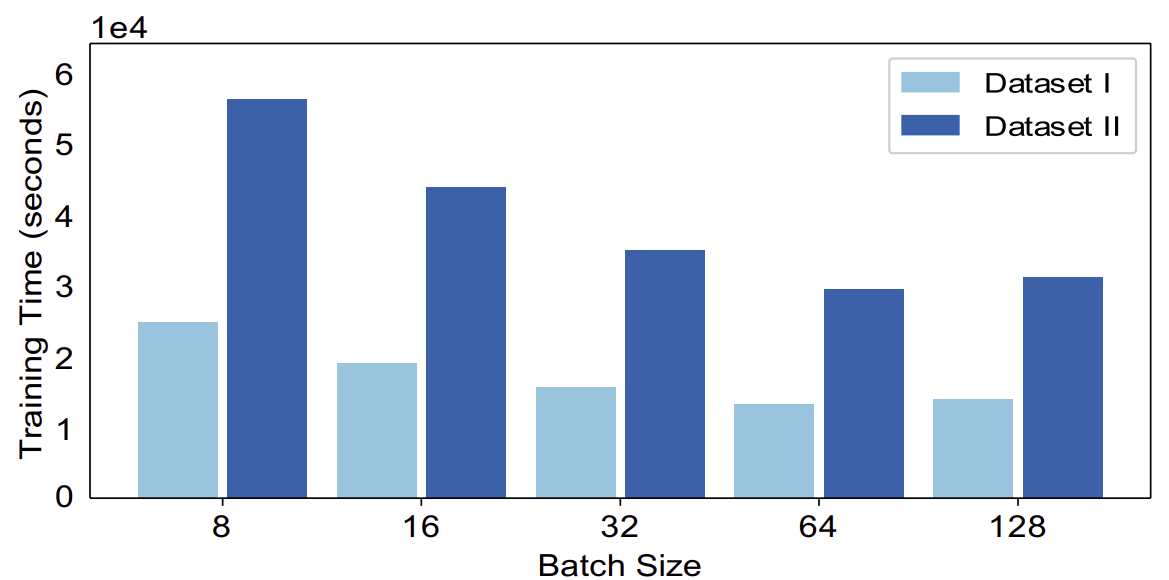
\includegraphics[scale=0.5]{MIT_1.PNG}
	\end{center}
	\caption{Thời gian đào tạo mô hình trên 4 GPU với các kích thước batch khác nhau. }
\end{figure}

\underline{Nhận xét}: thời gian đào tạo với epoch bằng 100 giảm khi kích thước batch tăng lên. Tuy nhiên, batch là 128 làm thời gian tính toán tăng lên 4.5\%  thời gian cần thiết để đào tạo mô hình. 

\begin{figure}[!h]
	\begin{center}
		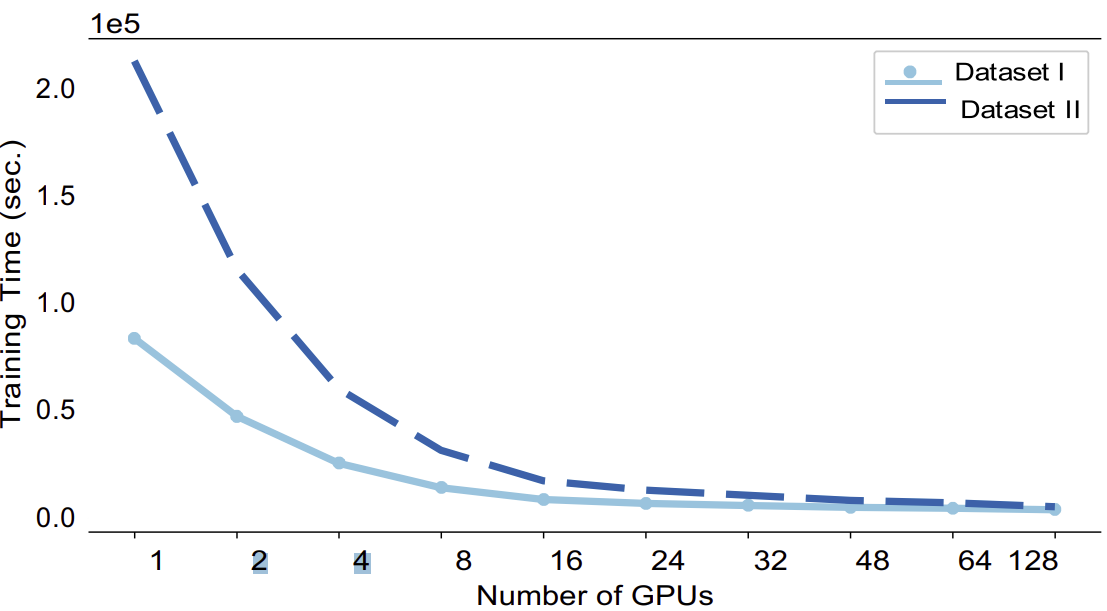
\includegraphics[scale=0.45]{MIT_2.PNG}
	\end{center}
	\caption{Thời gian đào tạo mô hình sử dụng GPU NVIDIA K80 trên nhiều nút máy tính. epoch = 100 }
\end{figure}


\begin{figure}[!h]
	\begin{center}
		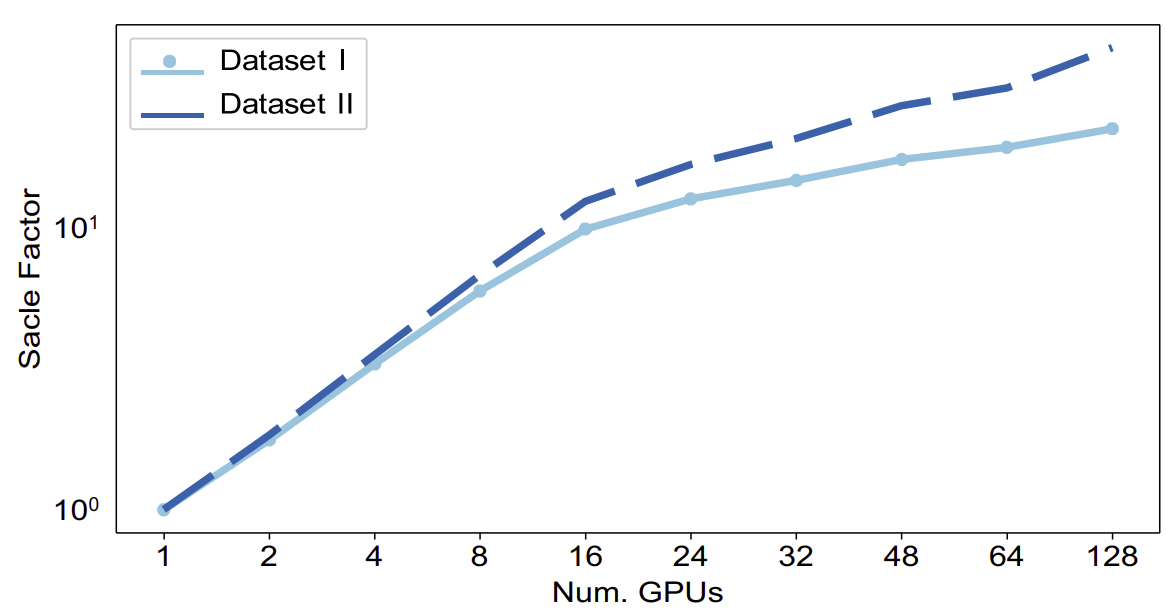
\includegraphics[scale=0.5]{MIT_3.PNG}
	\end{center}
	\caption{Tăng tốc đào tạo khi sử dụng mô hình song song. epoch = 100 }
\end{figure}

\begin{figure}[!h]
	\begin{center}
		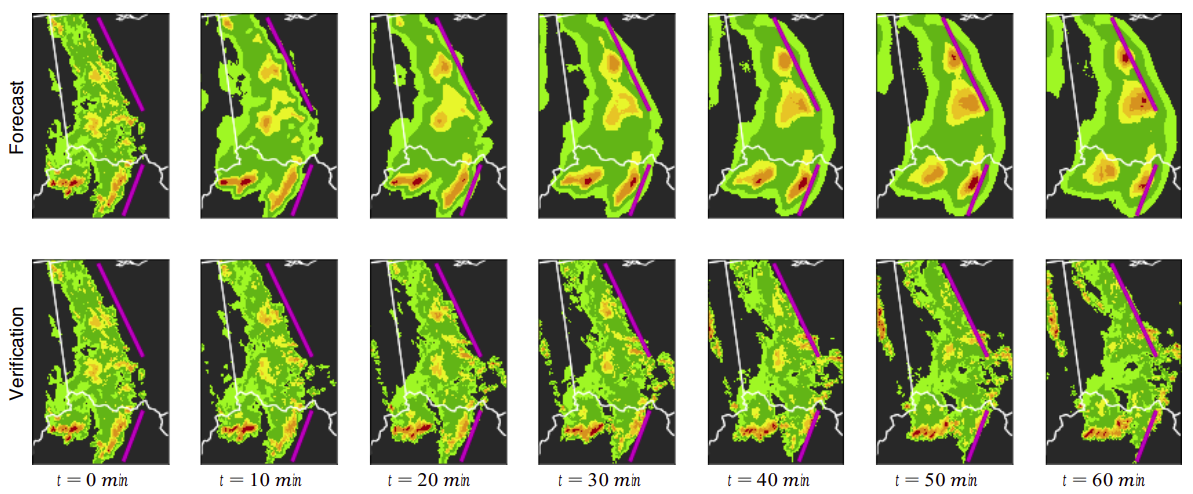
\includegraphics[scale=0.62]{MIT_4.PNG}
	\end{center}
	\caption{Trích dẫn kết quả dự báo của bài báo }
\end{figure}


\newpage
%%====================

\section{Kết quả chương trình Demo}
Mặc dù đã rất nỗ lực, tuy nhiên do rào cản quá lớn về phần cứng cũng như sức ép về thời gian nên em chưa thể hoàn thành việc chuyển đổi chương trình từ tập trung sang phân tán. Do vậy, trong phần kết quả này em xin được trình bày một chương trình Demo phần nào thể hiện được sự đào tạo phân tán là như thế nào.\\

Quá trình đào tạo mô hình được thực hiện trên Ubutu với thư viện được sử dụng để phân tán là TensorFlow. \\

Ở đây, do không có điều kiện về phần cứng nên em chỉ có thể \textbf{demo} chương trình trên \textbf{1 Laptop} bằng cách tạo các cổng (port) và coi mỗi cổng là một nút. Các nút sẽ giao tiếp với nhau thông qua giao thức TCP/IP

\lstset{language=Python}
\lstset{frame=lines}
\lstset{caption={Hàm tạo ra các tiến trình (processes)}}
\lstset{label={lst:code_direct}}
\lstset{basicstyle=\footnotesize}
\begin{lstlisting}
Import subprocess

subprocess.Popen('python3 asyn_distributed_tf.py --job_name "ps" --task_index 0',    	shell  = True)
subprocess.Popen('python3 asyn_distributed_tf.py --job_name "worker" --task_index_0',  shell  = True)
subprocess.Popen('python3 asyn_distributed_tf.py --job_name "worker" --task_index 1',  shell  = True)
subprocess.Popen('python3 asyn_distributed_tf.py --job_name "worker" --task_index 2',  shell  = True)
\end{lstlisting}

Khi chạy tới đoạn code của mình, mỗi process sẽ gọi tới mã nguồn và truyền tham số (ví dụ truyền số thứ tự của worker,..)

\lstset{language=Python}
\lstset{frame=lines}
\lstset{caption={Khởi tạo các cổng}}
\lstset{label={lst:code_direct}}
\lstset{basicstyle=\footnotesize}
\begin{lstlisting}
parameter_servers = ["localhost:2222"]
workers = [ "localhost:2223", "localhost:2224",'localhost: 2225']
cluster = tf.train.ClusterSpec({"ps":parameter_servers, "worker":workers})
\end{lstlisting}

Như vậy, nếu khởi tạo các nút thành công nghĩa là các cổng 2222 (server) và 2223, 2224, 2225 (worker) phải được khởi tạo và được mở.\\

Ở đây, sau khi chạy chương trình và kiểm tra em đã tìm thấy các cổng trên, tất cả đều đang trong trạng thái họa động.

\begin{figure}[!h]
	\begin{center}
		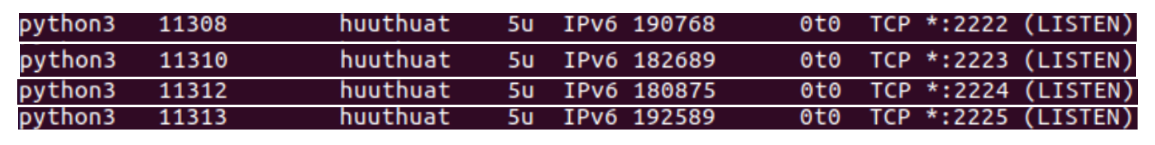
\includegraphics[scale=0.65]{IP.PNG}
	\end{center}
	\caption{Các cổng 2222, 2223, 2224, 2225 đã được khởi tạo và đang hoạt động}
\end{figure}

Trong chương trình Demo này, em đã chạy chương trình trong 2 trường hợp:  có 1 worker và có 3 worker để so sánh hiệu quả của việc đào tạo phân tán.\\

\begin{figure}[!h]
	\begin{center}
		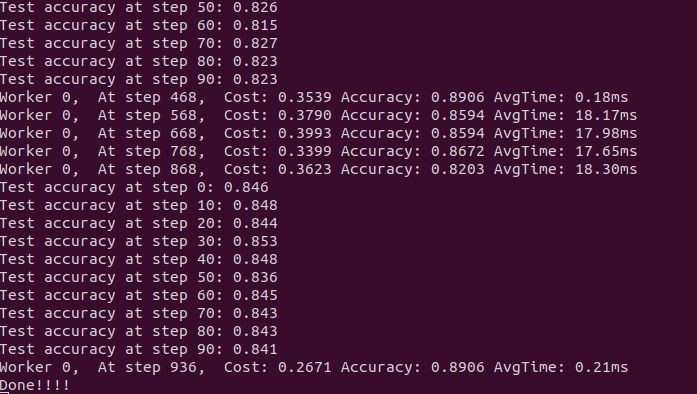
\includegraphics[scale=0.615]{Dis_1.PNG}
	\end{center}
	\caption{Đào tạo mô hình với 1 worker2}
\end{figure}

\begin{figure}[!h]
	\begin{center}
		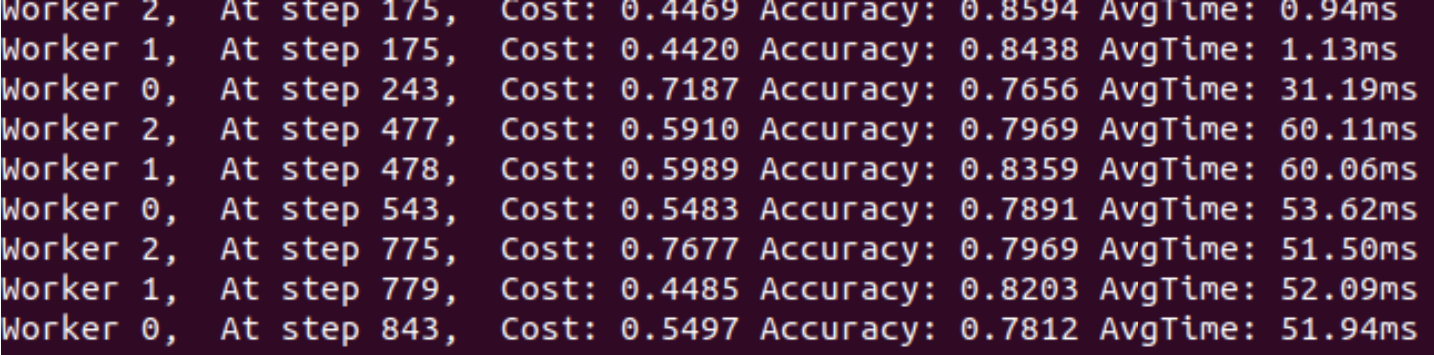
\includegraphics[scale=0.5]{Dis_2.PNG}
	\end{center}
	\caption{Đào tạo mô hình với 3 workers}
\end{figure}

\underline{Nhận xét}: 
\begin{enumerate}[-]
	\item Số bước khi sử dụng 3 workers là ít \textbf{hơn 1 chút} so với khi sử dụng 1 worker. Điều này cho thấy được \textbf{phần nào} đó sự hiệu quả của đào tạo phân tán.
	\item Tuy vậy, ta có thể dễ thấy rằng đồ chính xác, thời gian chạy trung bình của mô hình phân tán là \textbf{không tốt} so với khi chạy với 1 worker. Lý do xảy ra điều này là do bản chất chạy phân tán của em vẫn là trên 1 máy... nghĩa là 3 workers vẫn sử dụng "chung" CPU... do đó thời gian chạy rất chậm.
\end{enumerate}

Trên đây là một số kết quả mà em rút ra được từ chương trình Demo của em. Mặc dù kết quả chạy của chương trình chưa làm nổi bật tính ưu việt của phương pháp đào tạo học sâu phân tán đối với một mô hình phức tạp. Tuy nhiên, với 2 kết quả được trích dẫn từ 2 bài báo rất uy tín em tin rằng phương pháp này là rất hiệu quả trong nhiều trường hợp.



\newpage
%%===============
\section{Kết luận}
\begin{enumerate}[-]
	\item Khi làm việc với các mô hình Deep Learning trên nền tảng dữ liệu lớn, em đã suy nghĩ về việc tăng tốc đào tạo mô hình bằng một cách nào đó. Tuy nhiên, em không biết đó là cách nào.
	\item Khi Thầy đưa ra đề tài mở về một chủ đề liên quan đến tính toán song song... em đã đưa ra câu hỏi: "Liệu có thể áp dụng chiến lược song song vào quá trình đào tạo mô hình Deep Learning hay không?". Và em đã bắt đầu đi tìm hiểu.
	\item Việc tìm hiểu chủ đề này thực sự là một thách thức rất lớn khi thời gian tìm hiểu chỉ khoảng 2 tuần, trong khi em vẫn phải đi thực tập vào ban ngày. Ngoài ra, chủ đề này ở các trang tiếng việt thì rất ít và có thể nói là không tồn tại. Có thể do việc xây dựng được một mô hình học sâu ở Việt Nam với một bộ dữ liệu lớn thường chỉ ở trong những tập đoàn lớn như VinAI, VinBigData, Viettel hay FPT... và họ thường đầu tư những giàn máy chuyên biệt để đào tạo mô hình.
	\item Do vậy, khi tìm hiểu em đã tìm một số papers nổi tiếng liên quan đến vấn đề này và rất nhiều trang web viết về nó. Đây thực sự là một chủ đề khó khi mà các paper đều có tính học thuật rất cao.
	\item Do thời gian có hạn, nên em chỉ có thể tìm hiểu một các tổng quan nhất về đào tạo song song các mô hình học sâu trong bài tiểu luận này. Đây thực sự là một vấn đề thú vị và em chắc chắn sẽ tiếp tục tìm hiểu và phát triển nó trong thời gian tiếp theo.
	\item Em xin chân thành cảm ơn Thầy đã tận tình hướng dẫn em trong học phần "Tính toán song song" vừa qua. Em mong rằng sẽ nhật được những đánh giá từ Thầy để em có thể rút kinh nghiệm và làm tốt hơn trong những bài tiểu luận, bài báo cáo hay trong những đồ án sắp tới.
\end{enumerate}



\newpage
%%=========================
\section*{Tài liệu tham khảo}
\addcontentsline{toc}{section}{Tài liệu tham khảo}

[1] TAL BEN-NUN and TORSTEN HOEFLER, ETH Zurich, Switzerland,\textit{Demystifying Parallel and Distributed Deep Learning: An In-Depth Concurrency Analysis}. \\

[2]Matthias Langer, Member, IEEE, Zhen He, Wenny Rahayu and Yanbo Xue, Member, \textit{Distributed Training of Deep Learning Models: A Taxonomic Perspective}. \\

[3] Jeffrey Dean, Greg S. Corrado, Rajat Monga, Kai Chen, Matthieu Devin, Quoc V. Le, Mark Z. Mao, Marc’Aurelio Ranzato, Andrew Senior, Paul Tucker, Ke Yang, Andrew Y. Ng \textit{Large Scale Distributed Deep Networks}. \\

[4] Vishakh Hegde, Sheema Usmani, \textit{Parallel and Distributed Deep Learning}.\\

[5] Feng Yan, Olatunji Ruwase, Yuxiong He, Trishul Chilimb, \textit{Performance Modeling and Scalability Optimization of Distributed Deep Learning Systems}\\

[6] Siddharth Samsi, Christopher J. Mattioli, Mark S. Veillette, \textit{Distributed Deep Learning for Precipitation Nowcasting}, MIT Lincoln Laboratory, Lexington, MA.\\

[7] Hao Zhang, \textit{Intro to Distributed Deep Learning Systems}. URL: https://petuum.medium.- com/intro-to-distributed-deep-learning-systems-a2e45c6b8e7\\

[8] Srikanth Machiraju, \textit{How to train your deep learning models in a distributed fashion}. URL: https://towardsdatascience.com/how-to-train-your-deep-learning-models-in-a-distributed-fashion-43a6f53f0484.\\

[9] Google Brand, \textit{Distributed training with TensorFlow}. URL: https://   www.tensorflow.org /guide/distributed\_training.


\end{document}


